%!TEX root = ../thesis.tex

\newpage

\appendix

\section{ Исходные данные}
\label{c:source_data}
% latex table generated in R 3.1.2 by xtable 1.7-4 package
% Tue Mar  3 10:11:27 2015
\begin{table}[H]
\centering
\begin{tabular}{rrr}
  \hline
 & year & temperature \\ 
  \hline
1 & 1975.00 & 20.20 \\ 
  2 & 1976.00 & 16.00 \\ 
  3 & 1977.00 & 17.70 \\ 
  4 & 1978.00 & 16.75 \\ 
  5 & 1979.00 & 17.50 \\ 
  6 & 1980.00 & 16.77 \\ 
  7 & 1981.00 & 19.80 \\ 
  8 & 1982.00 & 19.00 \\ 
  9 & 1983.00 & 21.40 \\ 
  10 & 1984.00 & 19.40 \\ 
  11 & 1985.00 & 20.40 \\ 
  12 & 1986.00 & 16.50 \\ 
  13 & 1987.00 & 17.10 \\ 
  14 & 1988.00 & 23.80 \\ 
  15 & 1989.00 & 19.90 \\ 
  16 & 1990.00 & 18.50 \\ 
  17 & 1991.00 & 23.00 \\ 
  18 & 1992.00 & 21.90 \\ 
  19 & 1993.00 & 18.00 \\ 
  20 & 1994.00 & 21.40 \\ 
  21 & 1995.00 & 18.90 \\ 
  22 & 1996.00 & 19.10 \\ 
  23 & 1997.00 & 21.00 \\ 
  24 & 1998.00 & 18.40 \\ 
  25 & 1999.00 & 23.50 \\ 
  26 & 2000.00 & 21.00 \\ 
  27 & 2001.00 & 24.20 \\ 
  28 & 2002.00 & 23.10 \\ 
  29 & 2003.00 & 18.00 \\ 
  30 & 2004.00 & 19.10 \\ 
  31 & 2005.00 & 20.00 \\ 
  32 & 2006.00 & 21.30 \\ 
  33 & 2007.00 & 19.40 \\ 
  34 & 2008.00 & 21.80 \\ 
  35 & 2009.00 & 21.90 \\ 
  36 & 2010.00 & 24.30 \\ 
  37 & 2011.00 & 22.80 \\ 
  38 & 2012.00 & 20.20 \\ 
   \hline
\end{tabular}
\caption{Исходные данные.} 
\label{table:source}
\end{table}


\newpage
\section{ Графические материалы}
\label{c:graphs}

\setcounter{figure}{0}

\begin{figure}[H]
	\center{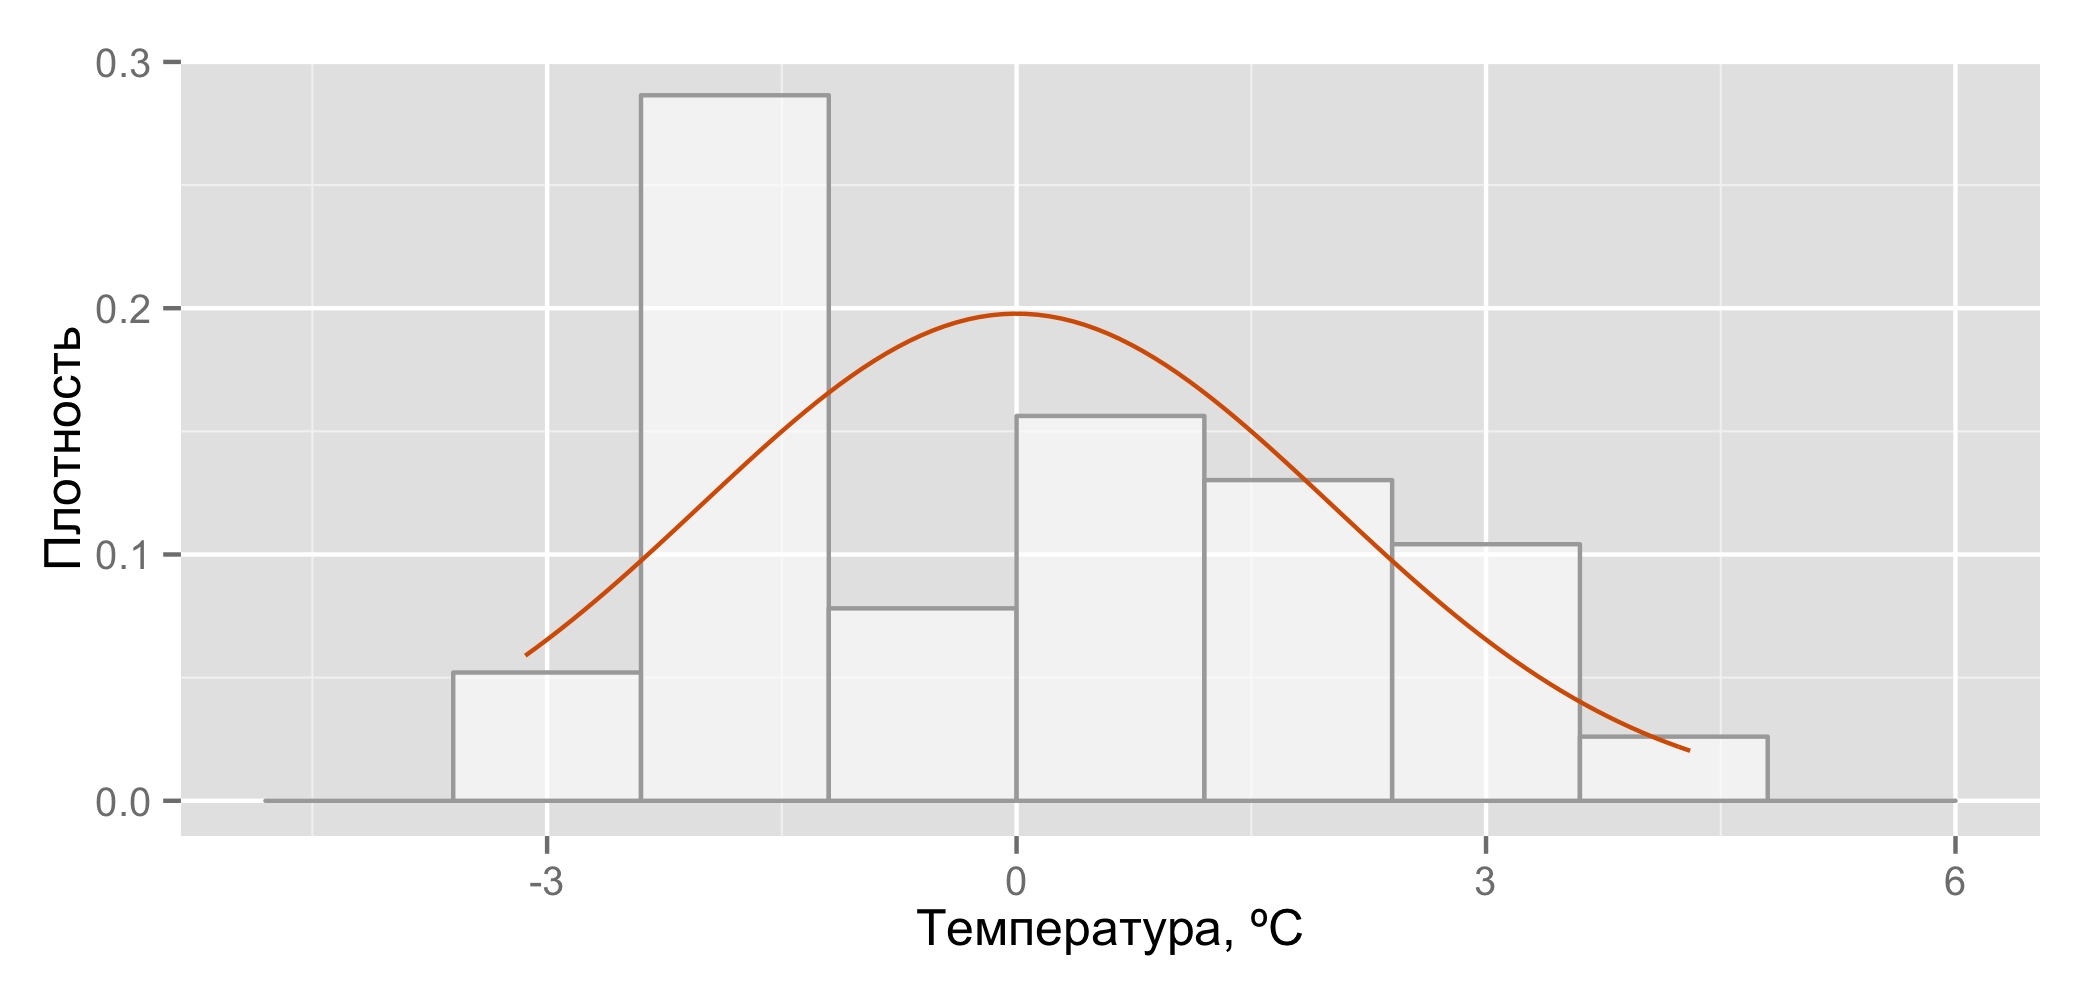
\includegraphics[width=0.9\linewidth]{../figures/residual/histogram.png}}
\caption{Гистограмма остатков с кривой плотности нормального распределения $\mathcal{N}(19.88, 4.92)$}
\label{img:resid_hist}
\end{figure}

\begin{figure}[H]
	\center{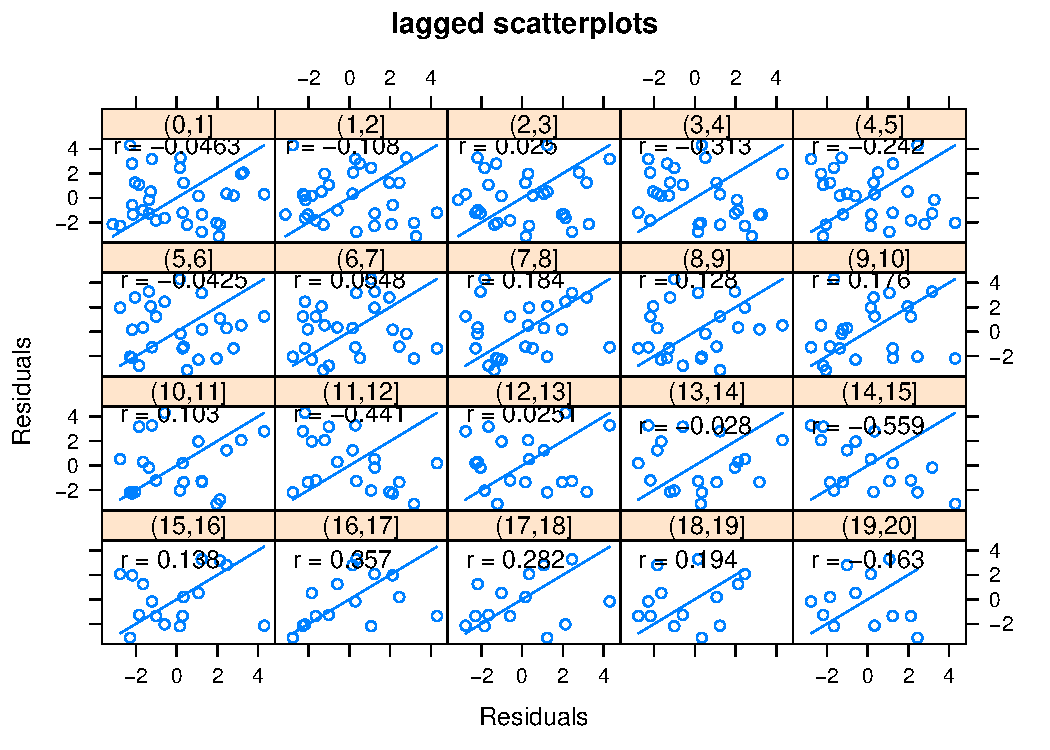
\includegraphics[width=0.9\linewidth]{../figures/residual/hscat.pdf}}
\caption{Диаграмма взаимного разброса}
\label{img:hscat}
\end{figure}

\begin{figure}[H]
	\center{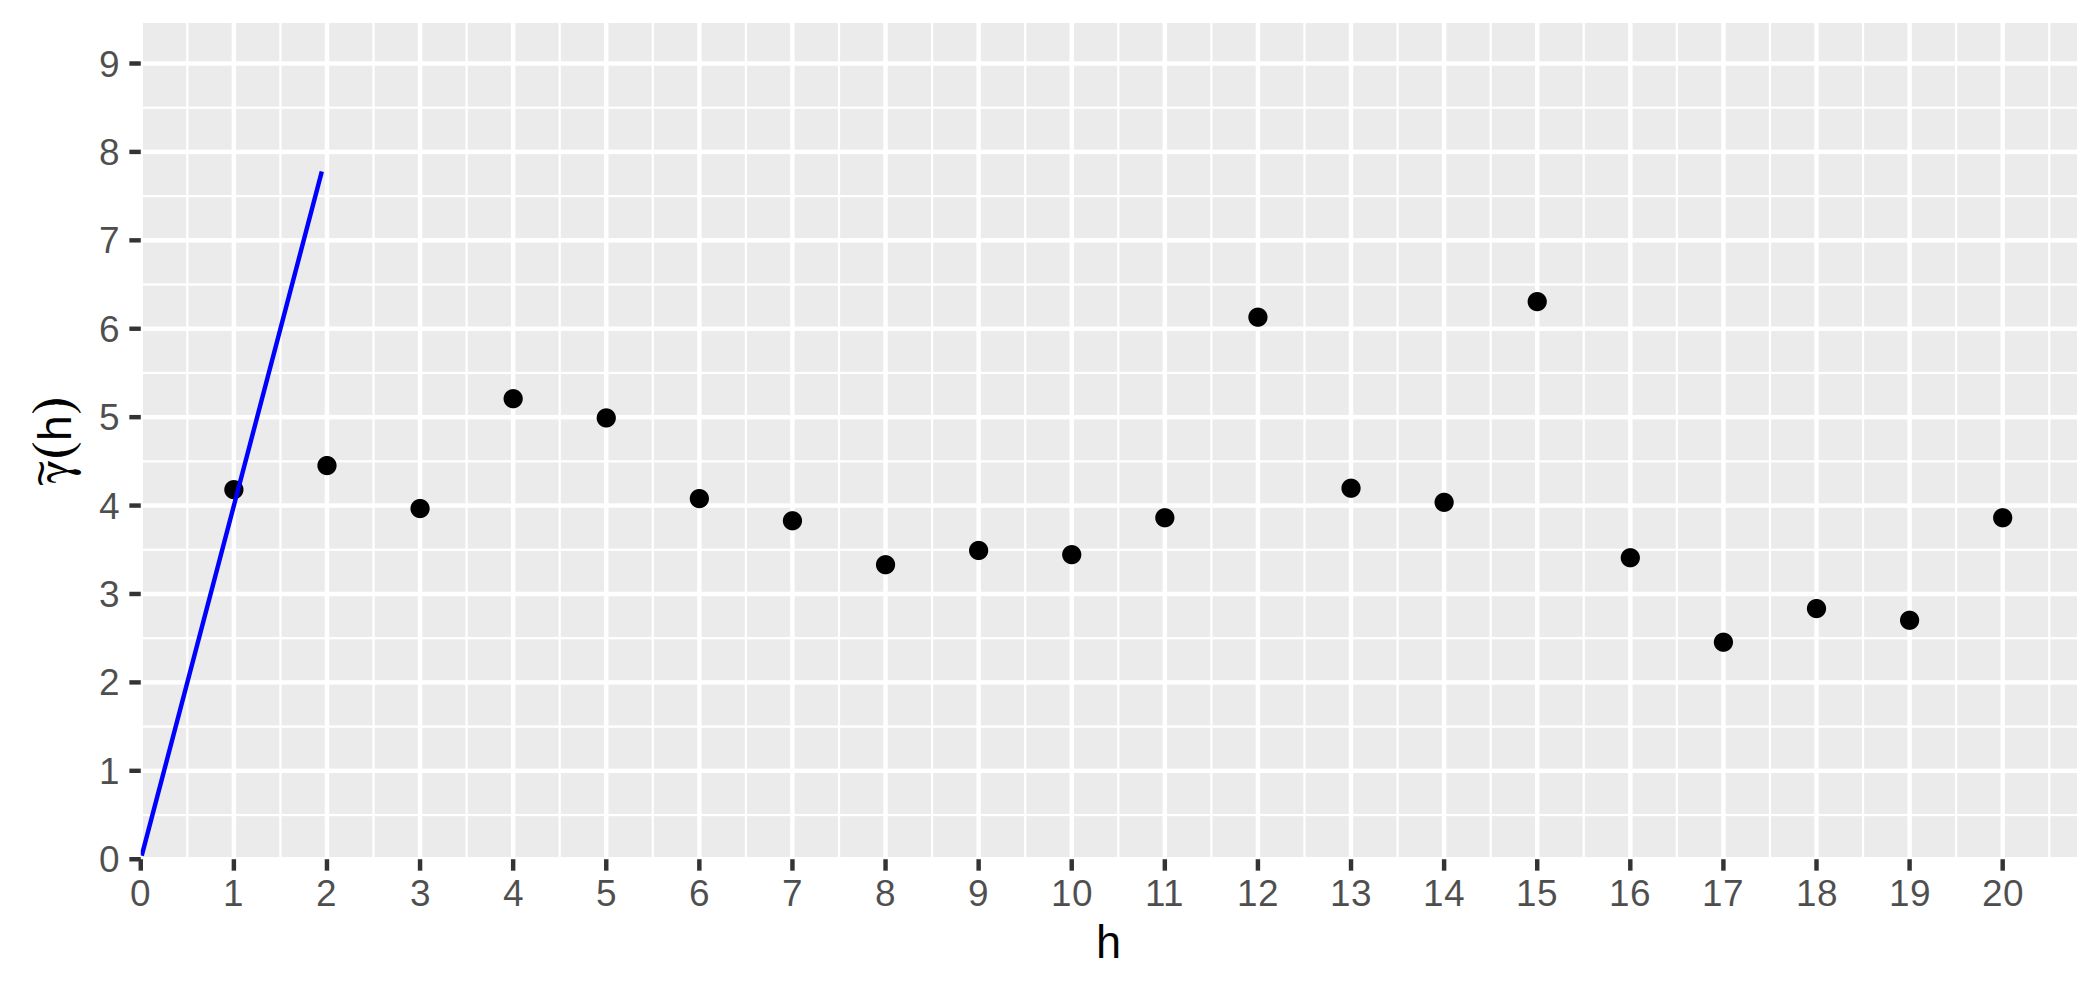
\includegraphics[width=0.8\linewidth]{../figures/variogram/lin-modeled.png}}
\caption{Семивариограмма и оценка $ \widehat{\gamma}_1(h) $}
\label{img:lin-modeled}
\end{figure}

\begin{figure}[H]
	\center{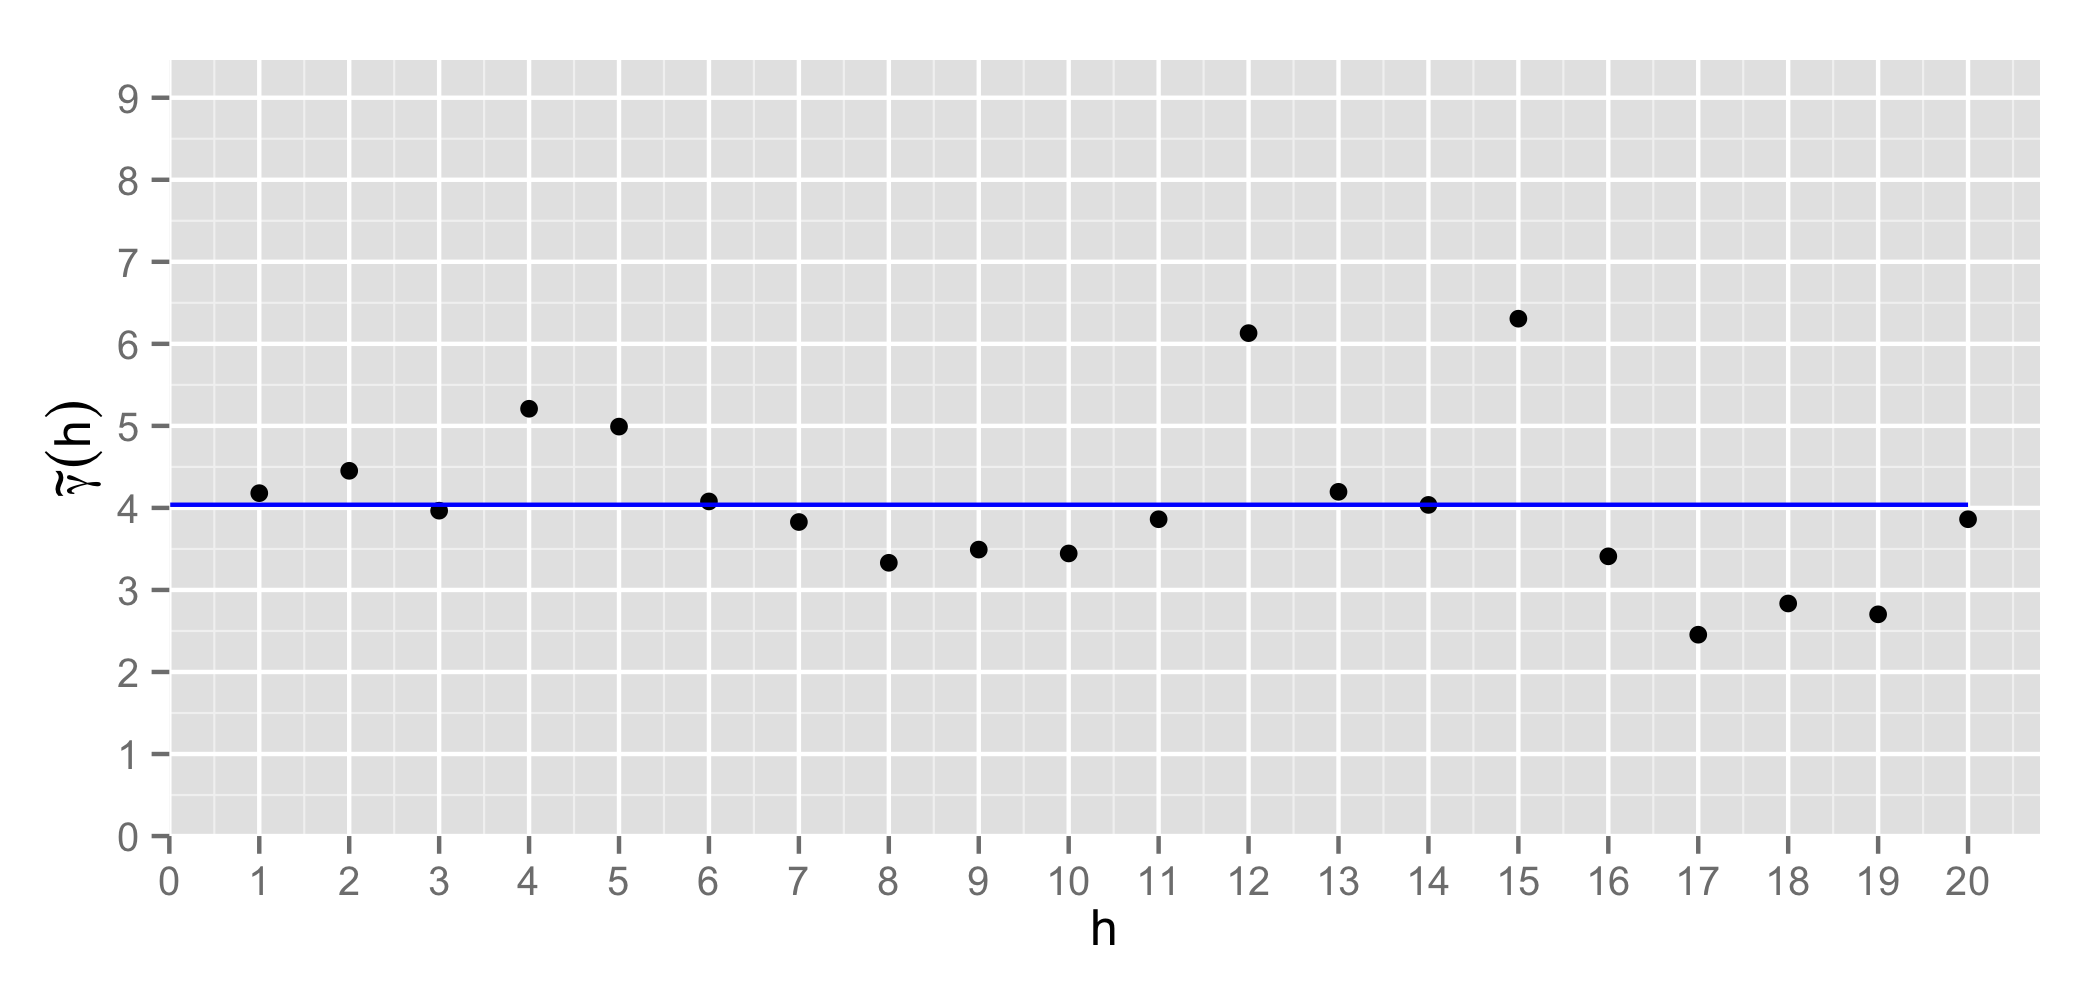
\includegraphics[width=0.8\linewidth]{../figures/variogram/lin-fit-modeled.png}}
\caption{Семивариограмма и оценка $ \widehat{\gamma}_2(h) $}
\label{img:lin-fit}
\end{figure}

\begin{figure}[H]
	\center{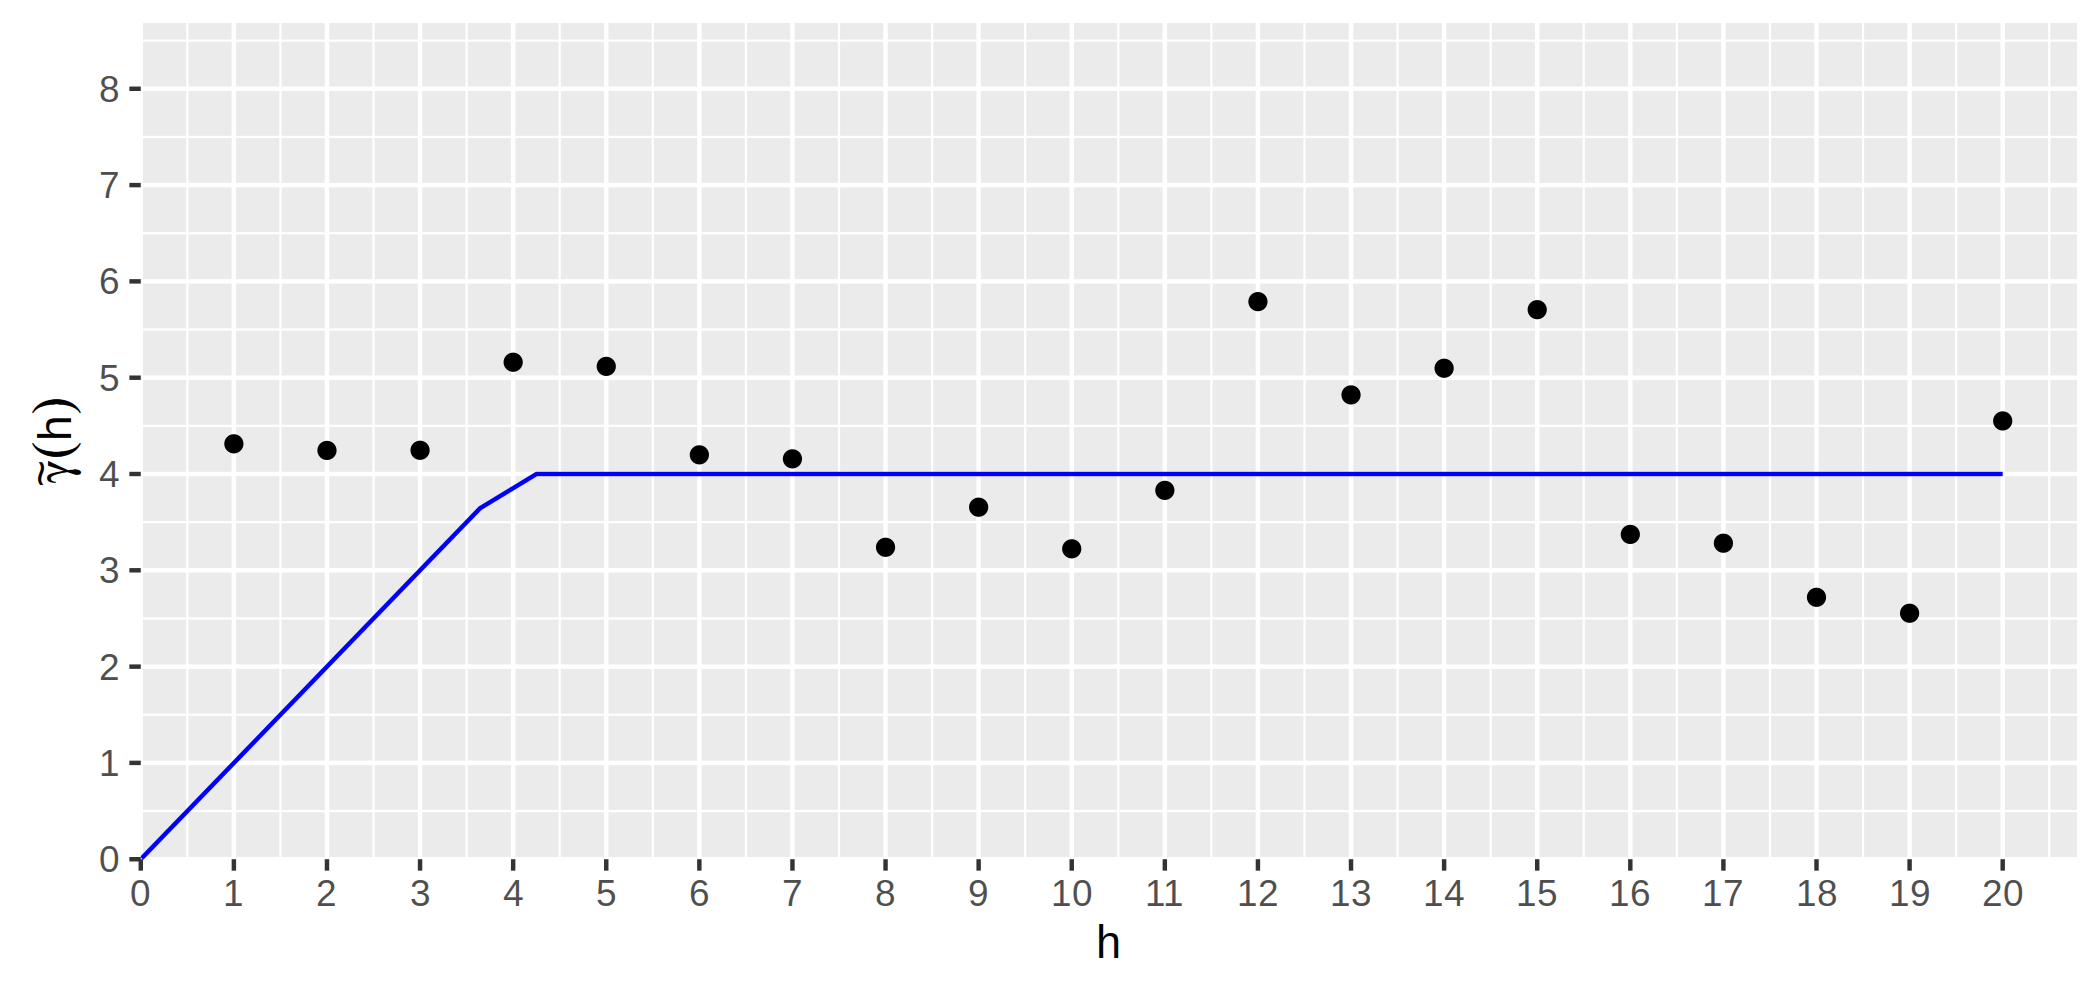
\includegraphics[width=0.8\linewidth]{../figures/variogram/lin-fit-cv-modeled.png}}
\caption{Семивариограмма и оценка $ \widehat{\gamma}_3(h) $}
\label{img:lin-fit-cv}
\end{figure}

\begin{figure}[H]
	\center{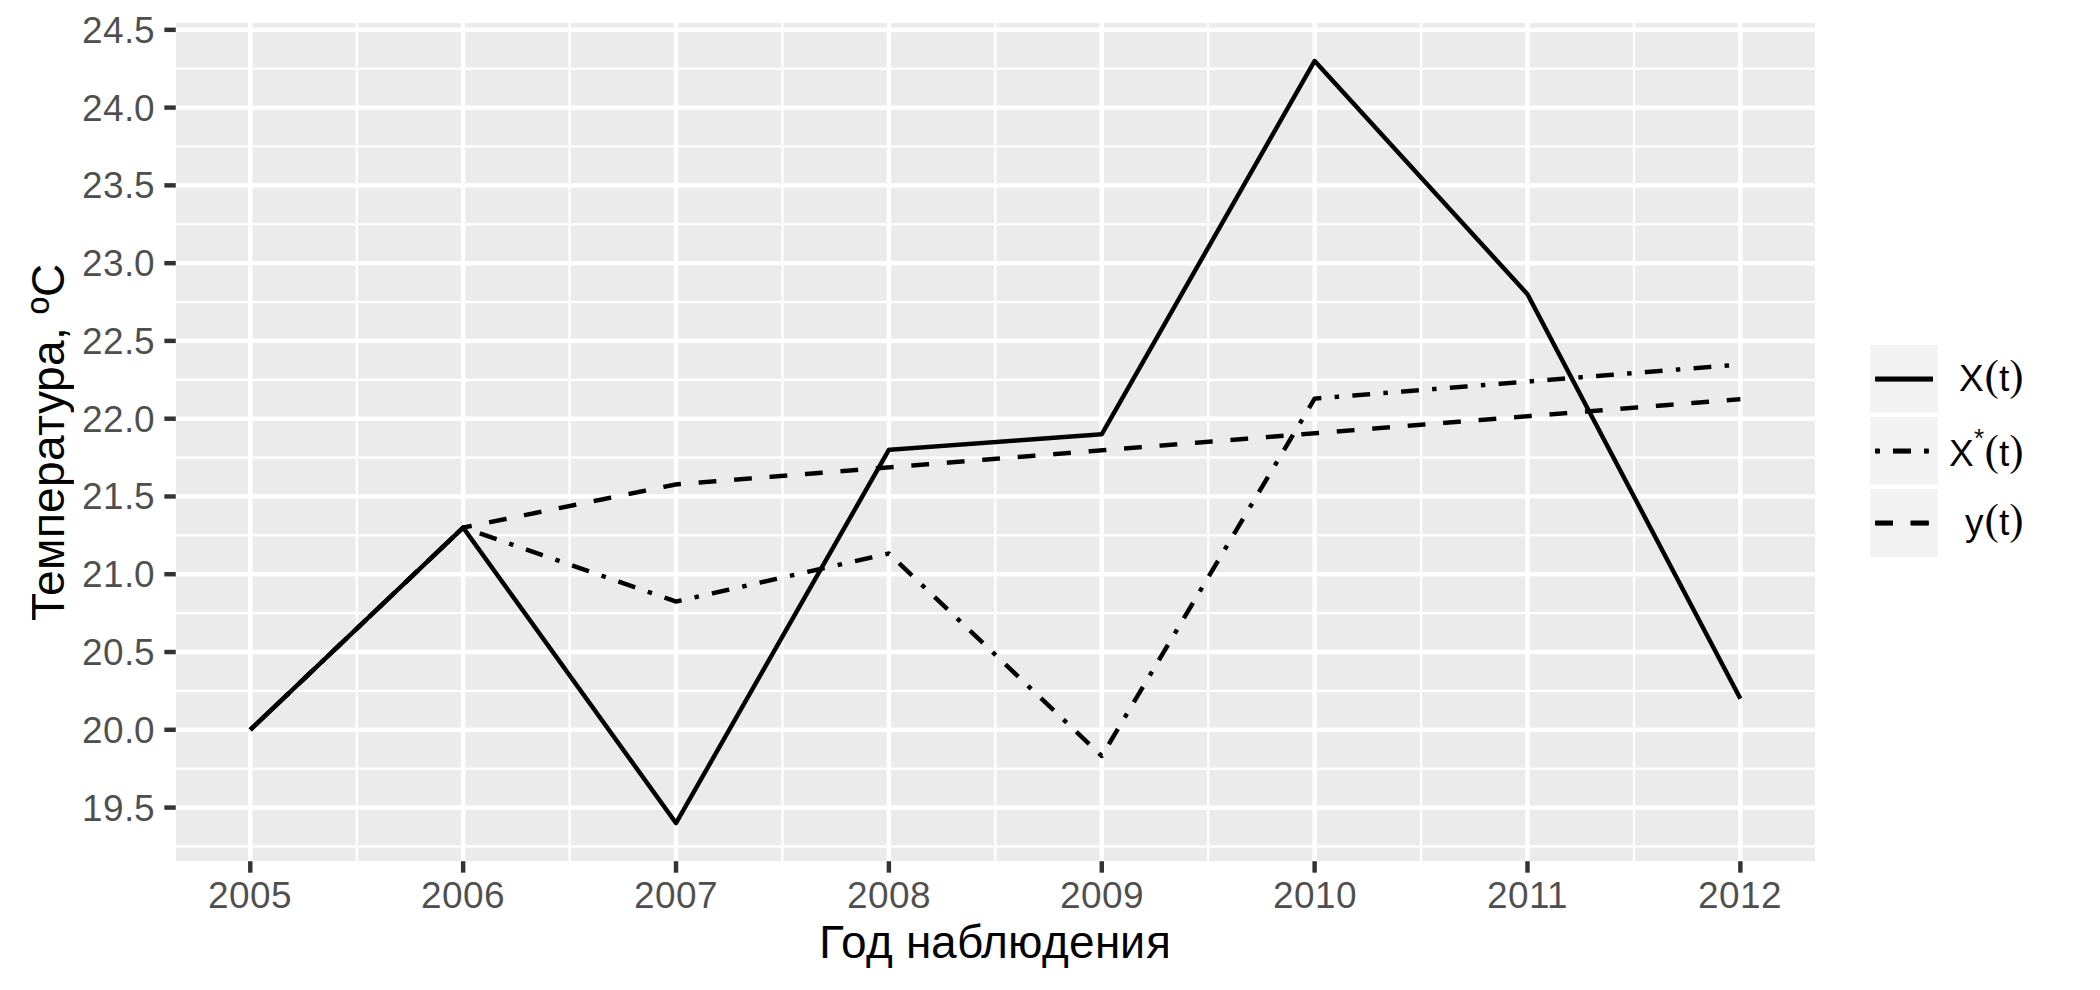
\includegraphics[width=0.8\linewidth]{../figures/variogram/lin-fit-cv-cross-prediction.png}}
\caption{Прогноз (модель $ \widehat{\gamma}_3(h) $)}
\label{img:lin-fit-cv-pred}
\end{figure}

\begin{figure}[H]
	\center{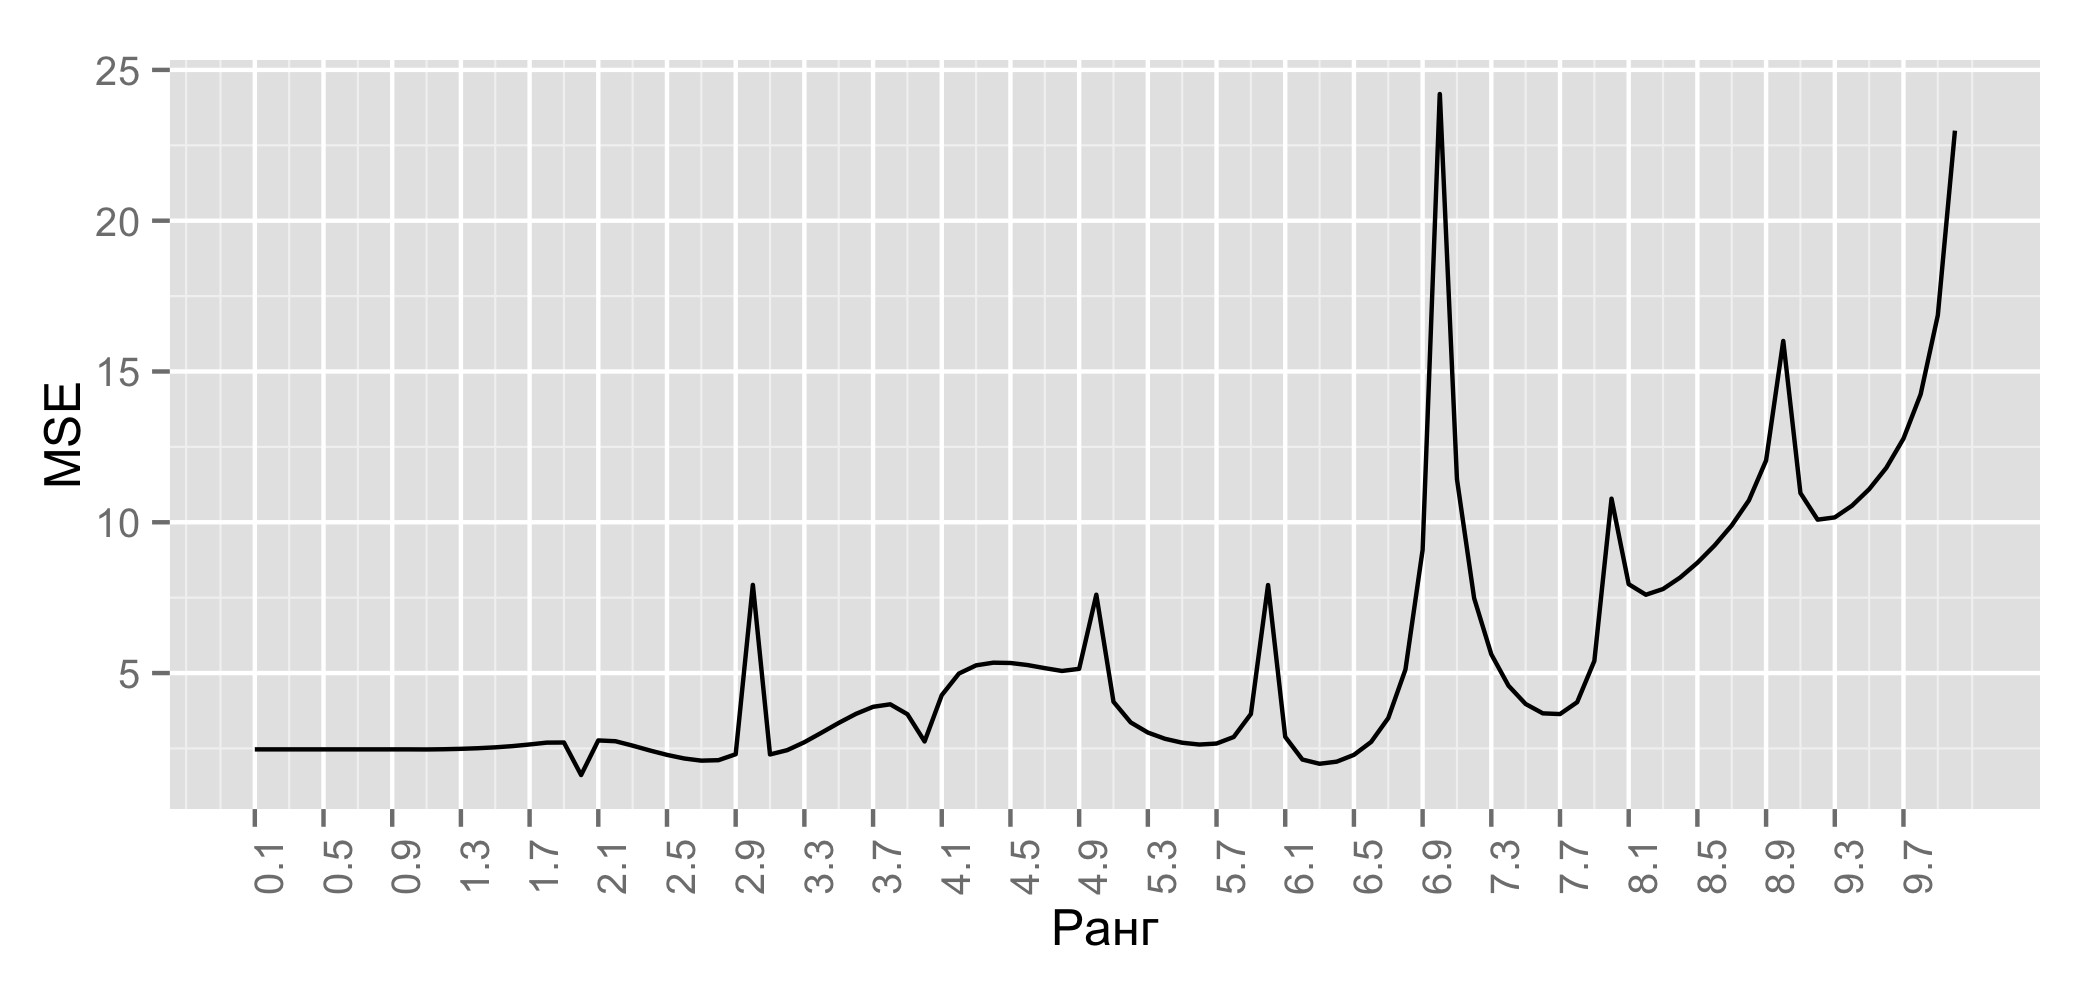
\includegraphics[width=0.8\linewidth]{../figures/variogram/lin-range-adapt.png}}
\caption{Зависимость качества линейной модели от значения ранга}
\label{img:lin-range-adapt}
\end{figure}

\begin{figure}[H]
	\center{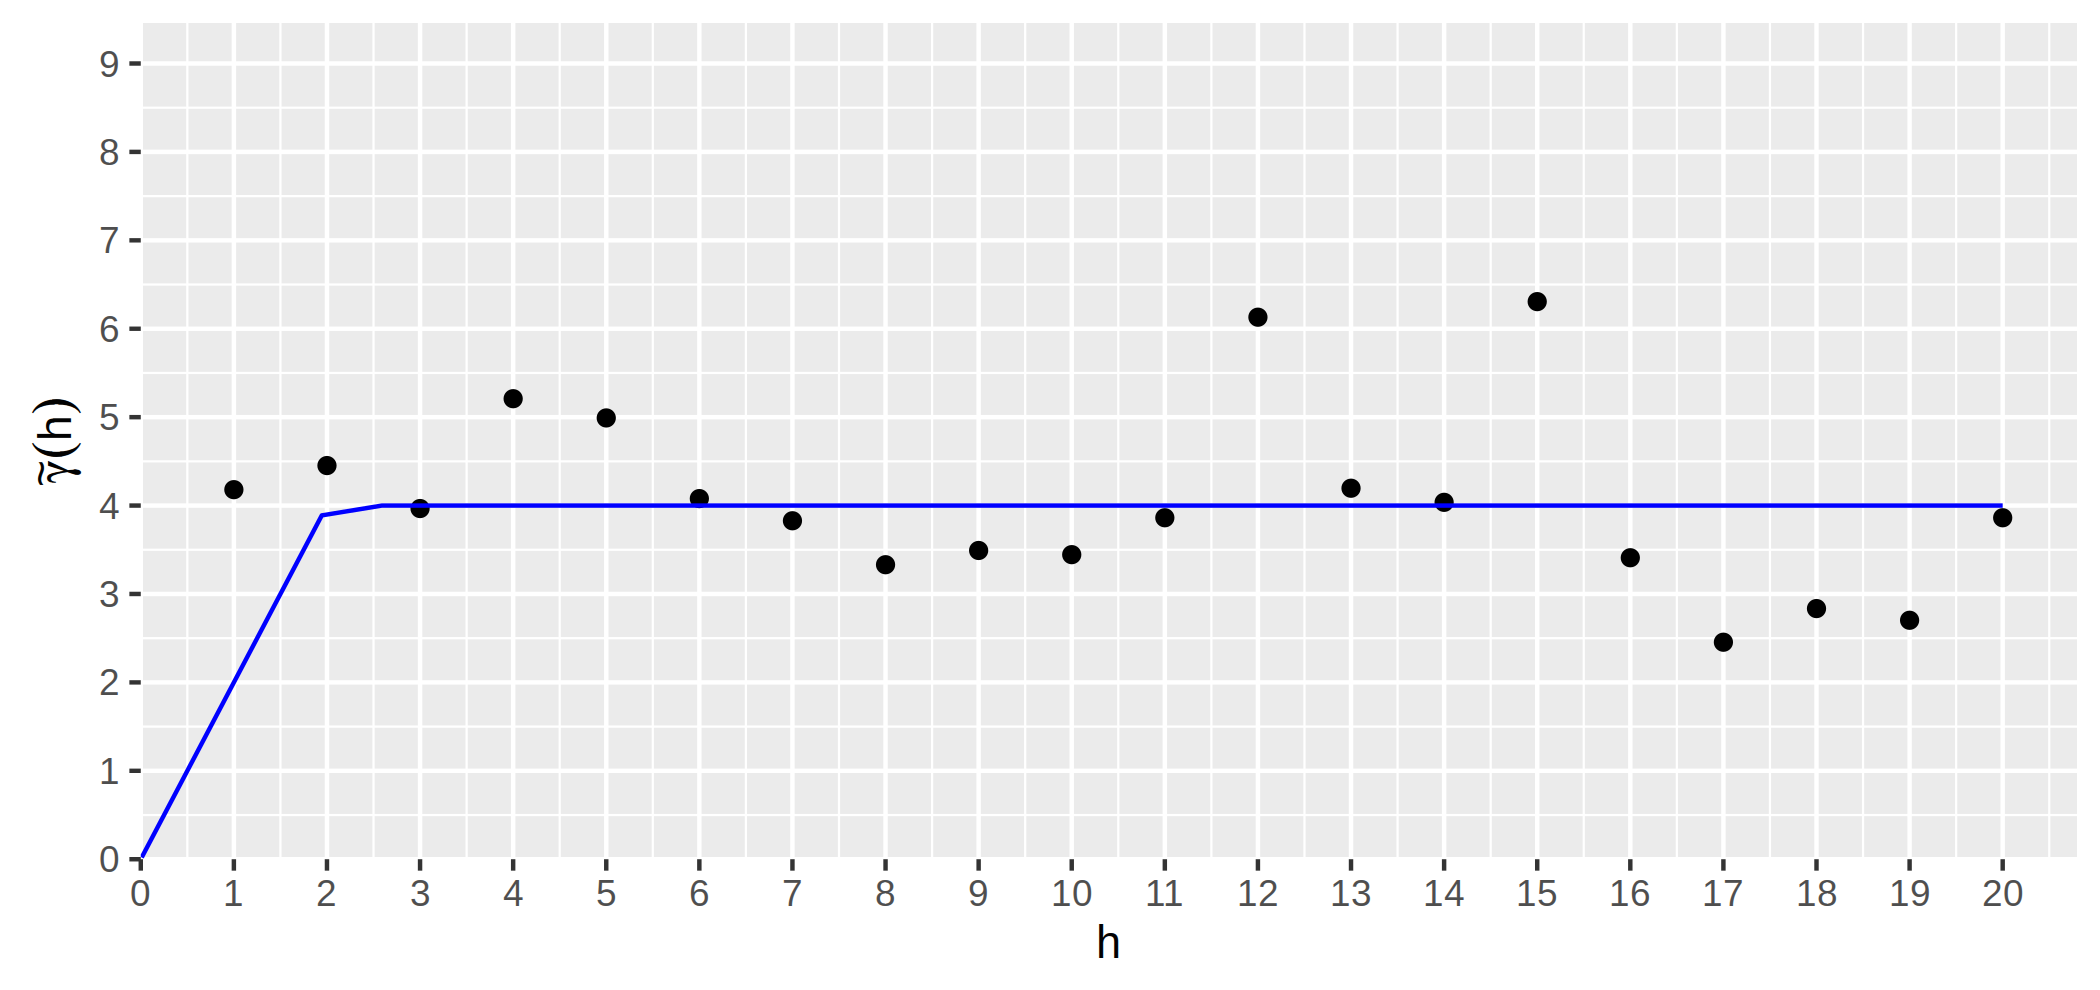
\includegraphics[width=0.8\linewidth]{../figures/variogram/lin-fit-adapt-modeled.png}}
\caption{Семивариограмма и оценка $ \widehat{\gamma}_4(h) $}
\label{img:lin-adapt-modeled}
\end{figure}

\begin{figure}[H]
	\center{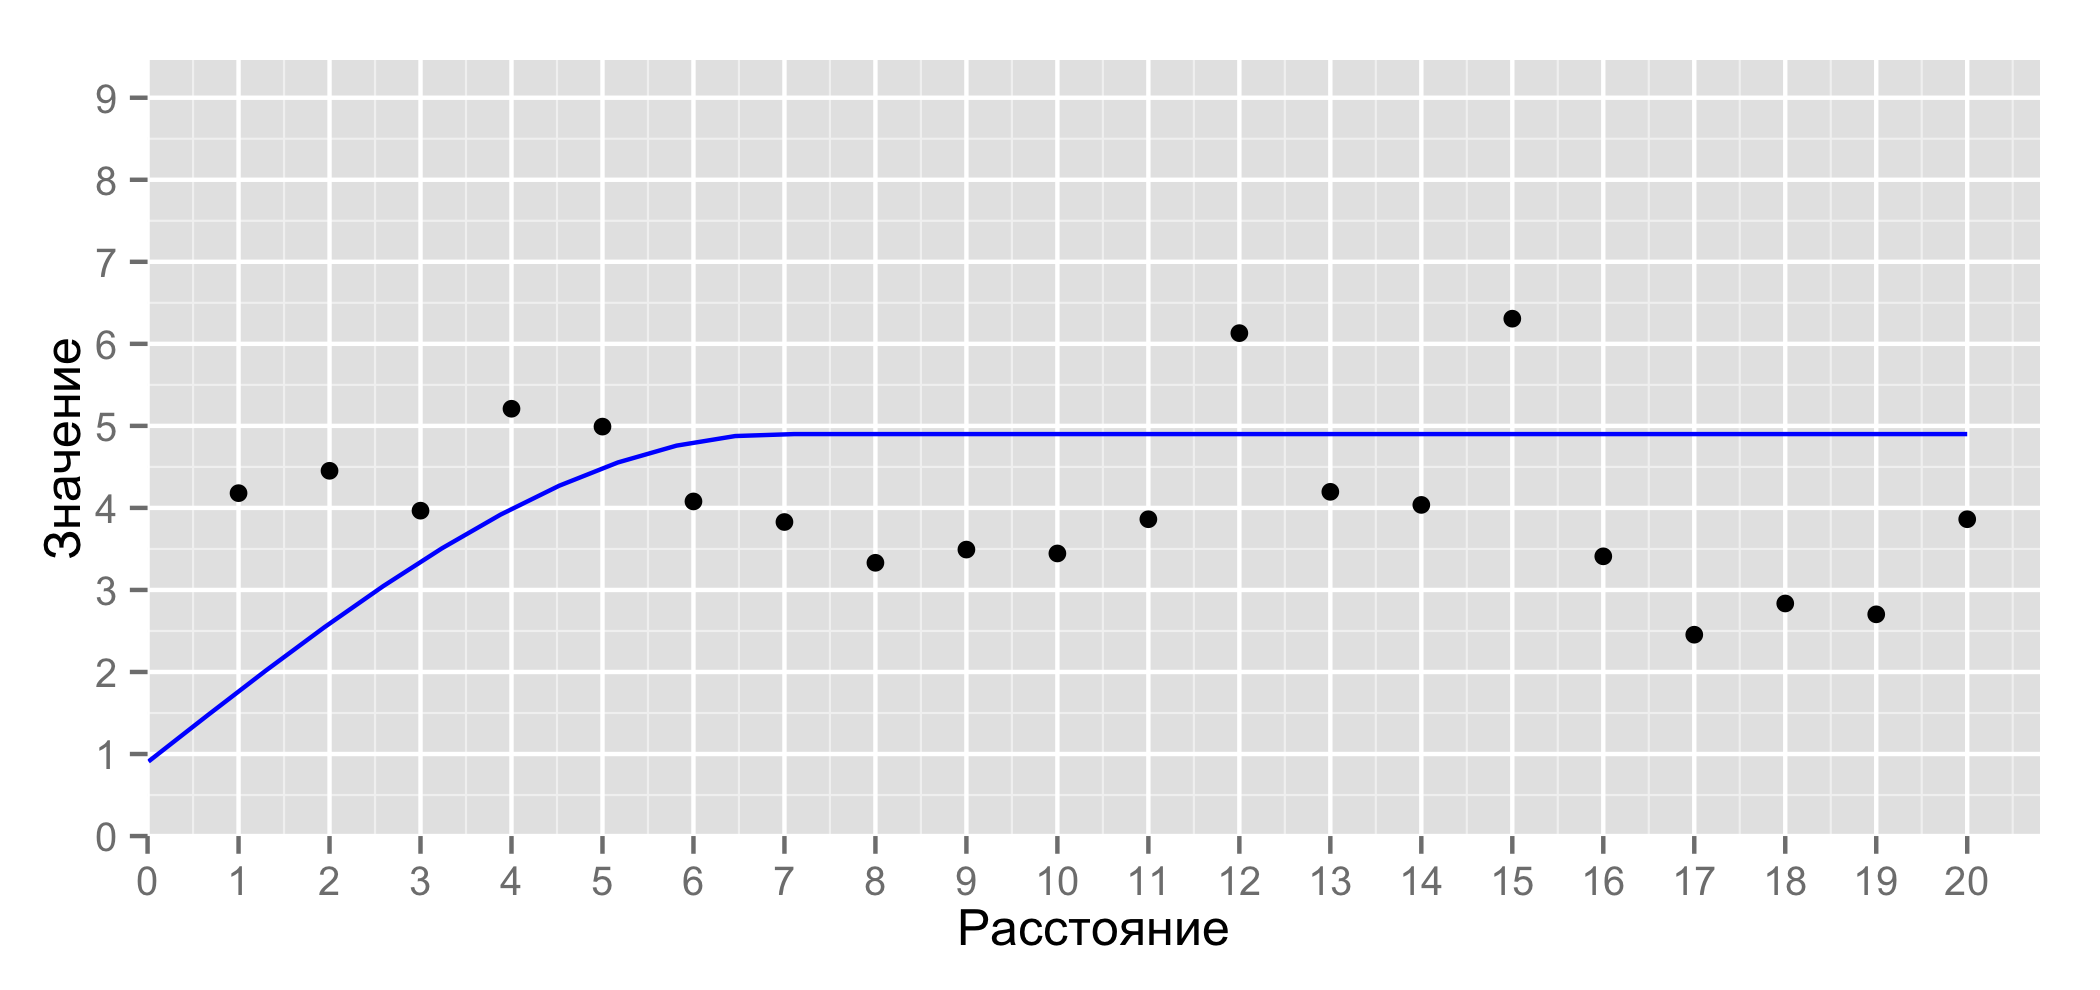
\includegraphics[width=0.8\linewidth]{../figures/variogram/sph-fit-adapt-modeled.png}}
\caption{Семивариограмма и оценка $ \widehat{\gamma}_5(h) $}
\label{img:sph-adapt-modeled}
\end{figure}

\begin{figure}[H]
	\center{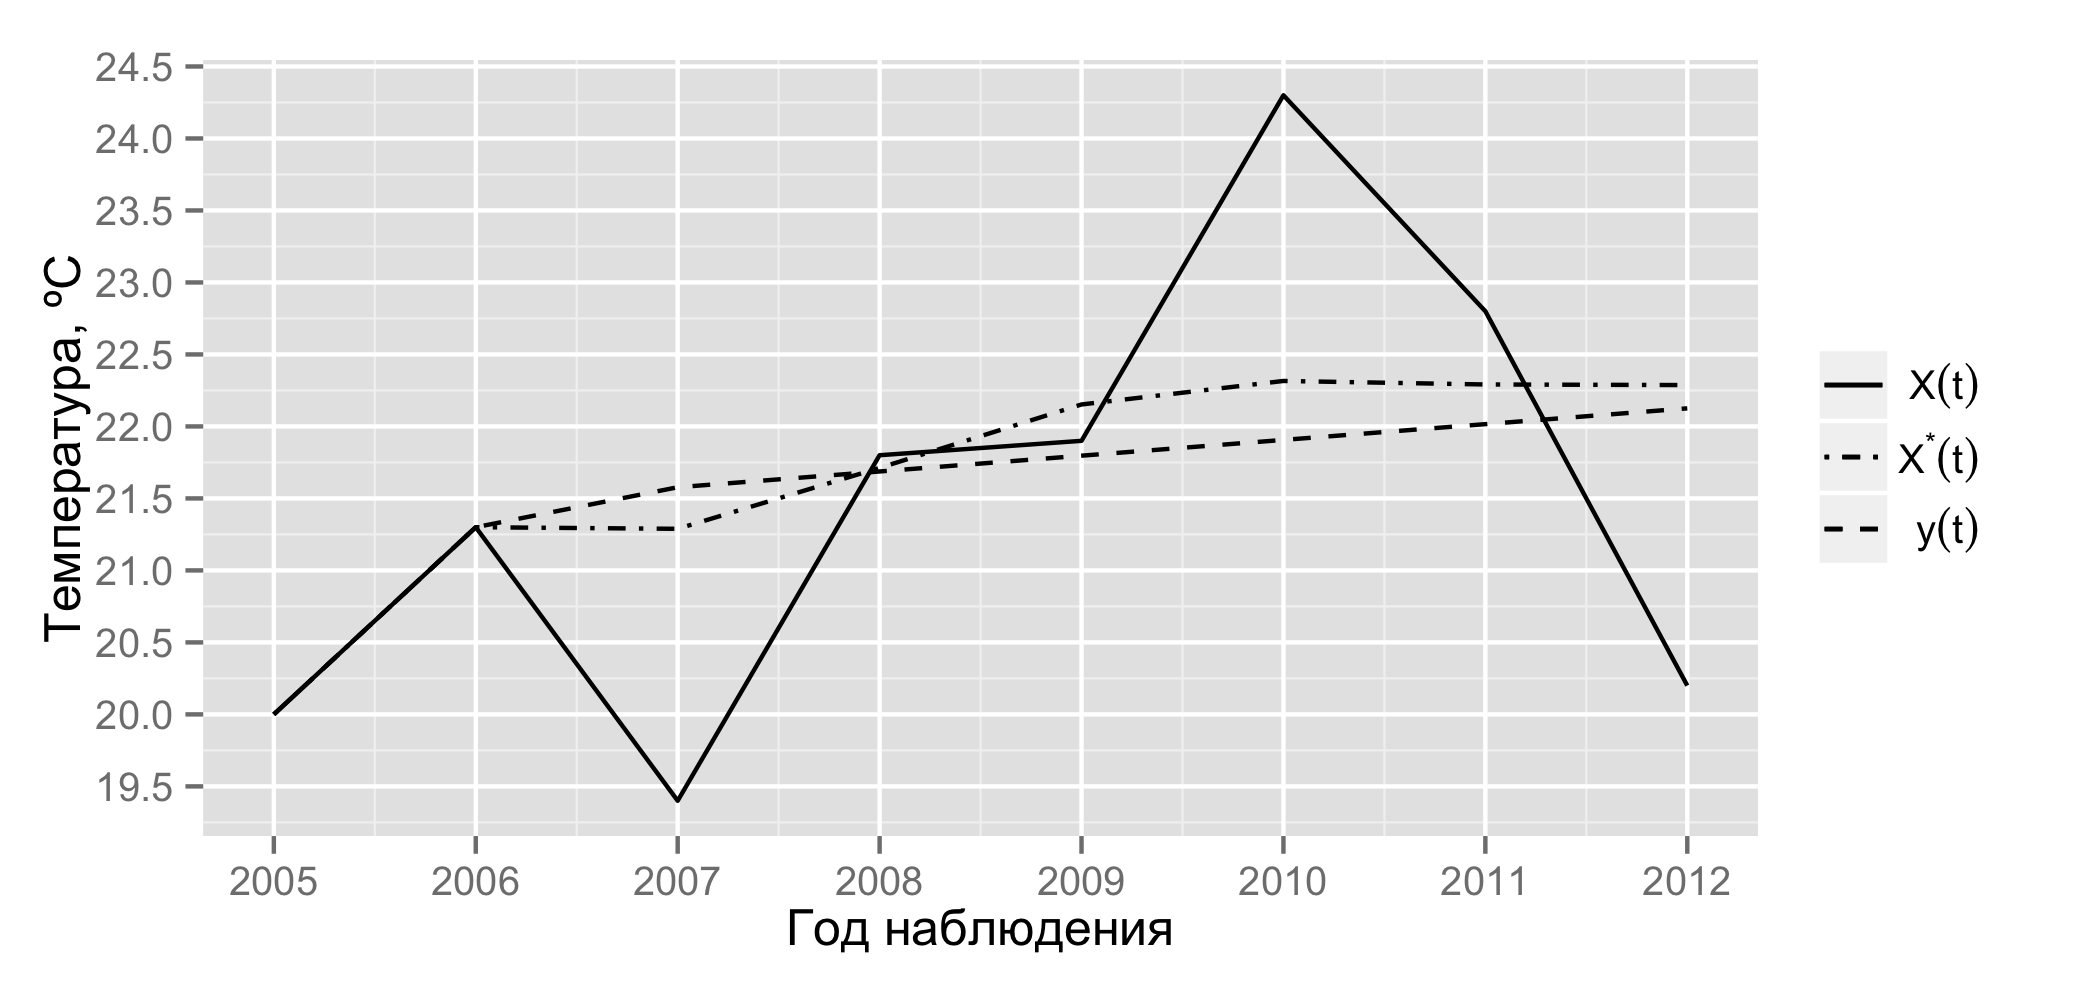
\includegraphics[width=0.8\linewidth]{../figures/variogram/sph-fit-adapt-cross-prediction.png}}
\caption{Прогноз (модель $ \widehat{\gamma}_5(h) $)}
\label{img:sph-adapt-pred}
\end{figure}

\begin{figure}[H]
	\center{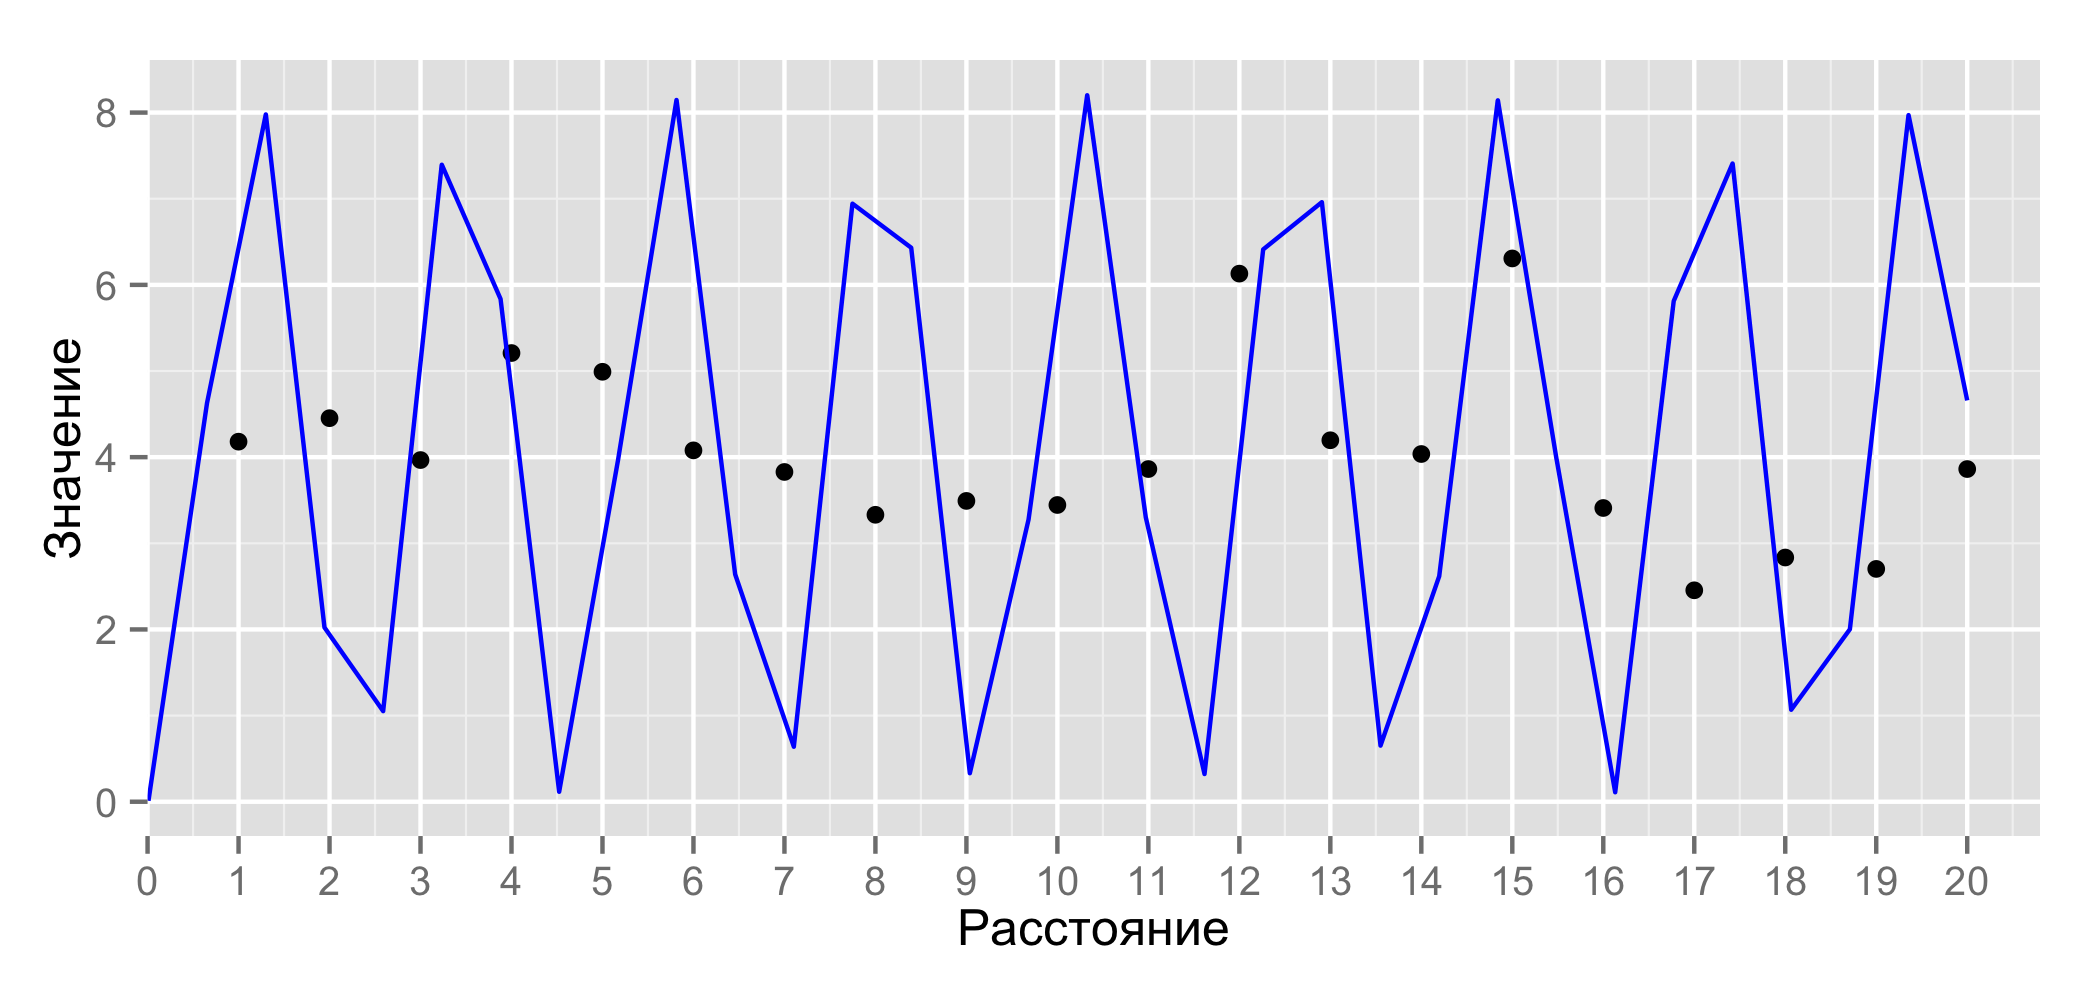
\includegraphics[width=0.8\linewidth]{../figures/variogram/per-fit-cv-modeled.png}}
\caption{Семивариограмма и оценка $ \widehat{\gamma}_6(h) $}
\label{img:per-cv-modeled}
\end{figure}

\begin{figure}[H]
\center{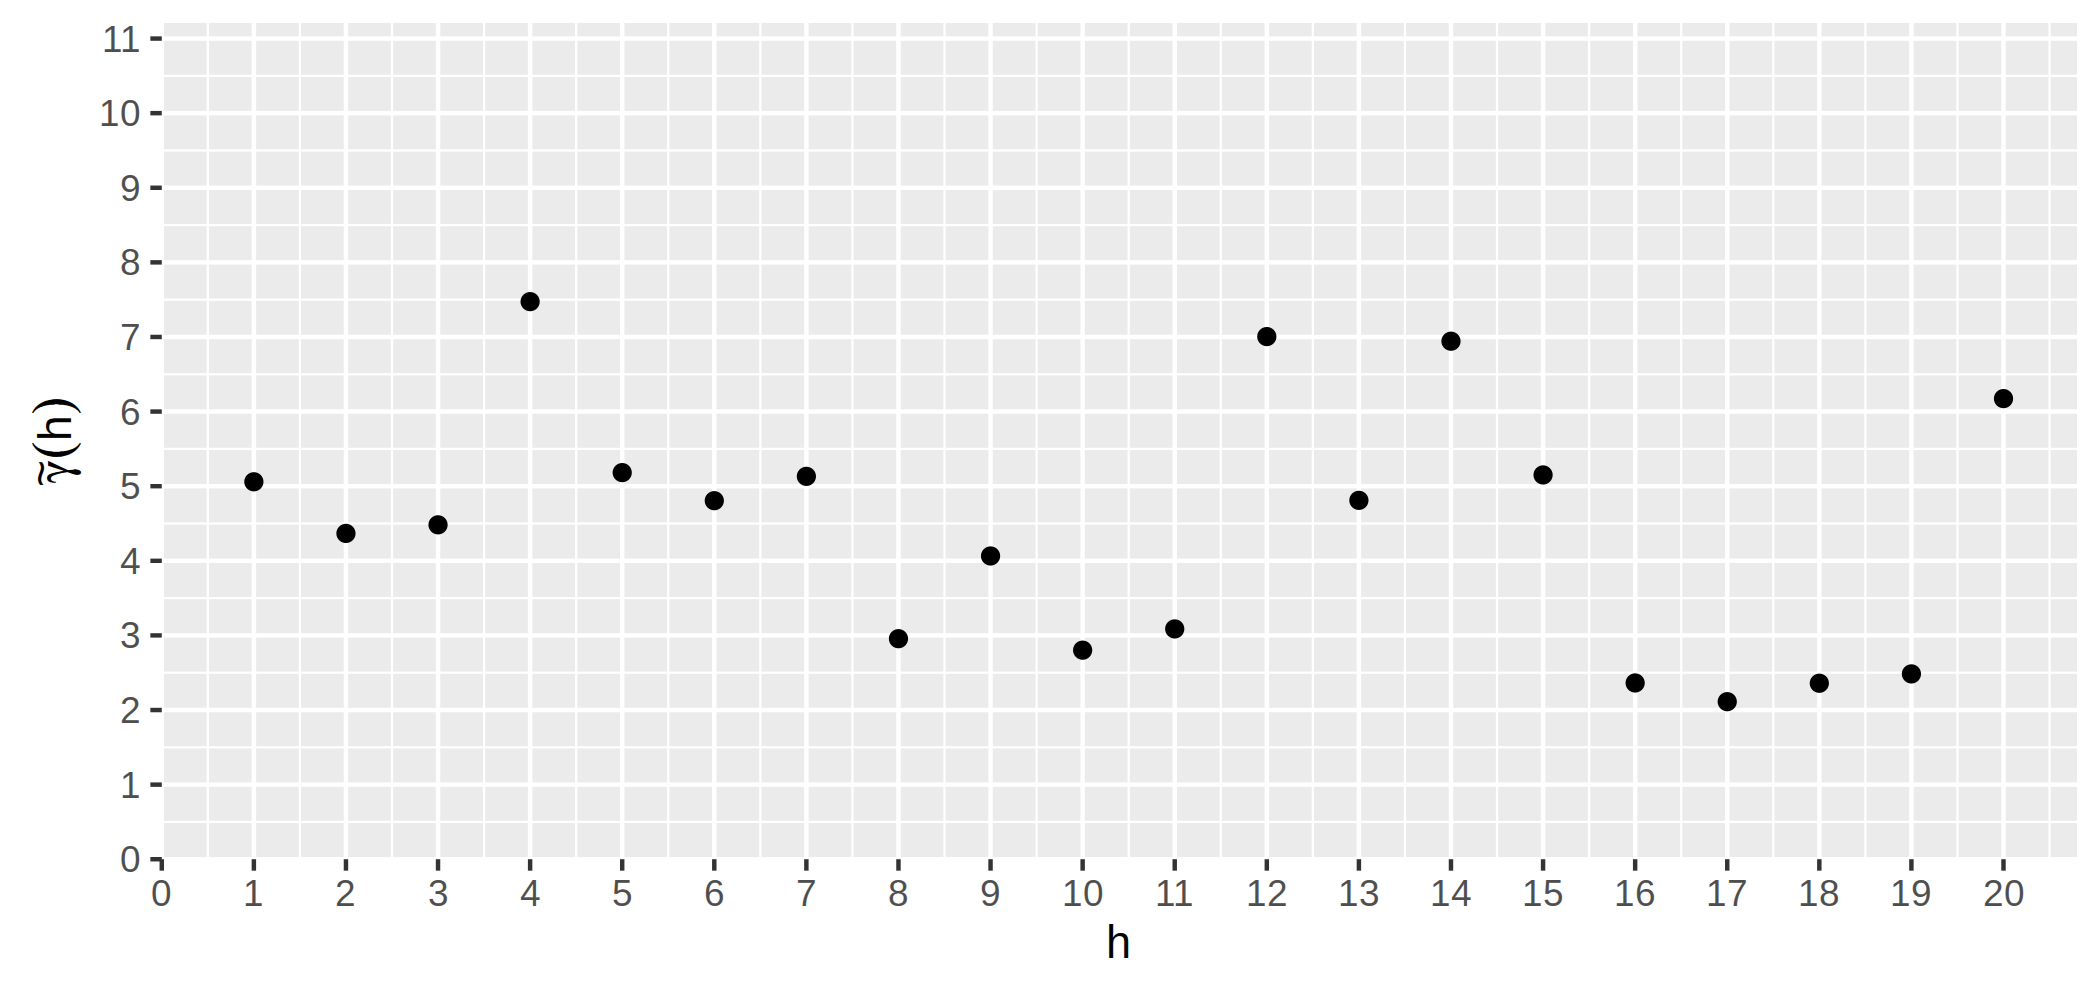
\includegraphics[width=0.8\linewidth]{../figures/variogram/robust-variogram.png}}
\caption{Оценка семивариограммы Кресси-Хокинса}
\label{img:robust-variogram}
\end{figure}

\begin{figure}[H]
\center{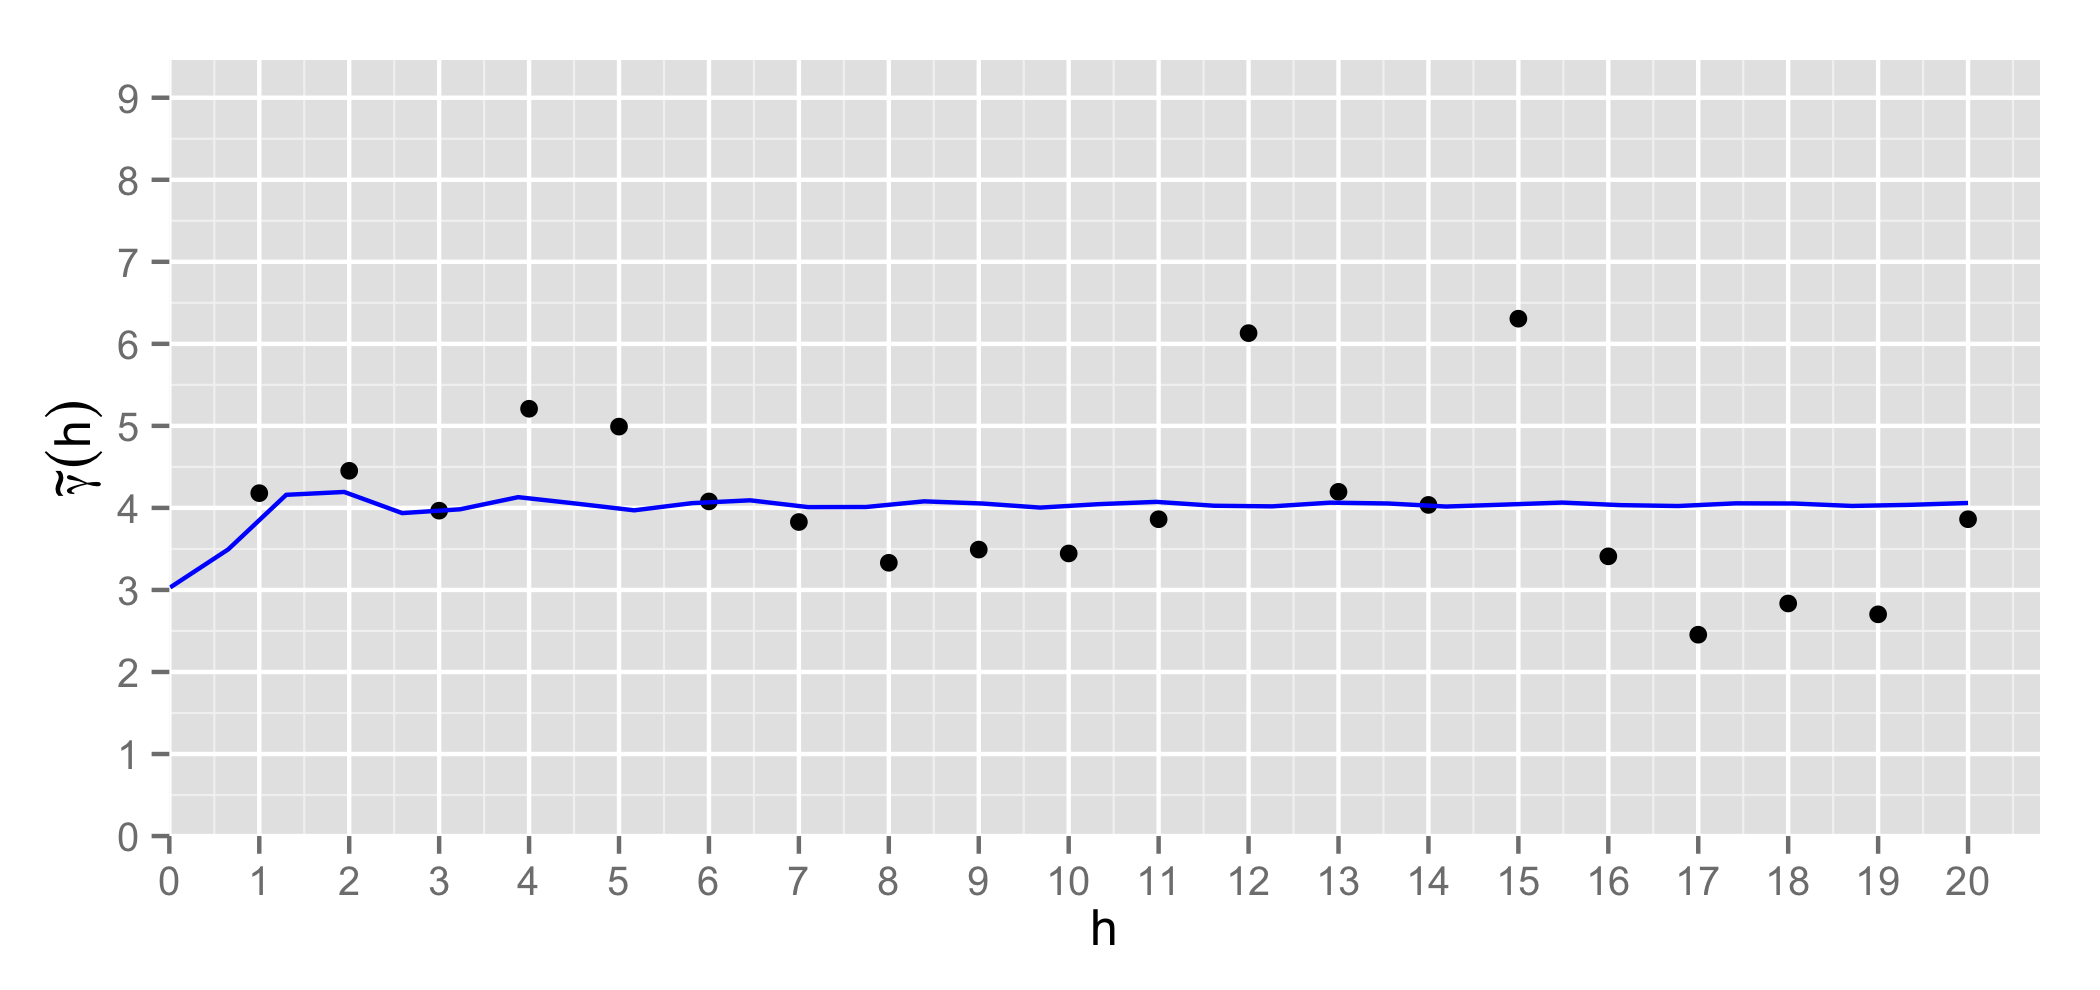
\includegraphics[width=0.8\linewidth]{../figures/variogram/auto-class-20-modeled.png}}
\caption{Семивариограмма и оценка $ \widehat{\gamma}_7(h) $}
\label{img:auto-class-modeled}
\end{figure}

\begin{figure}[H]
\center{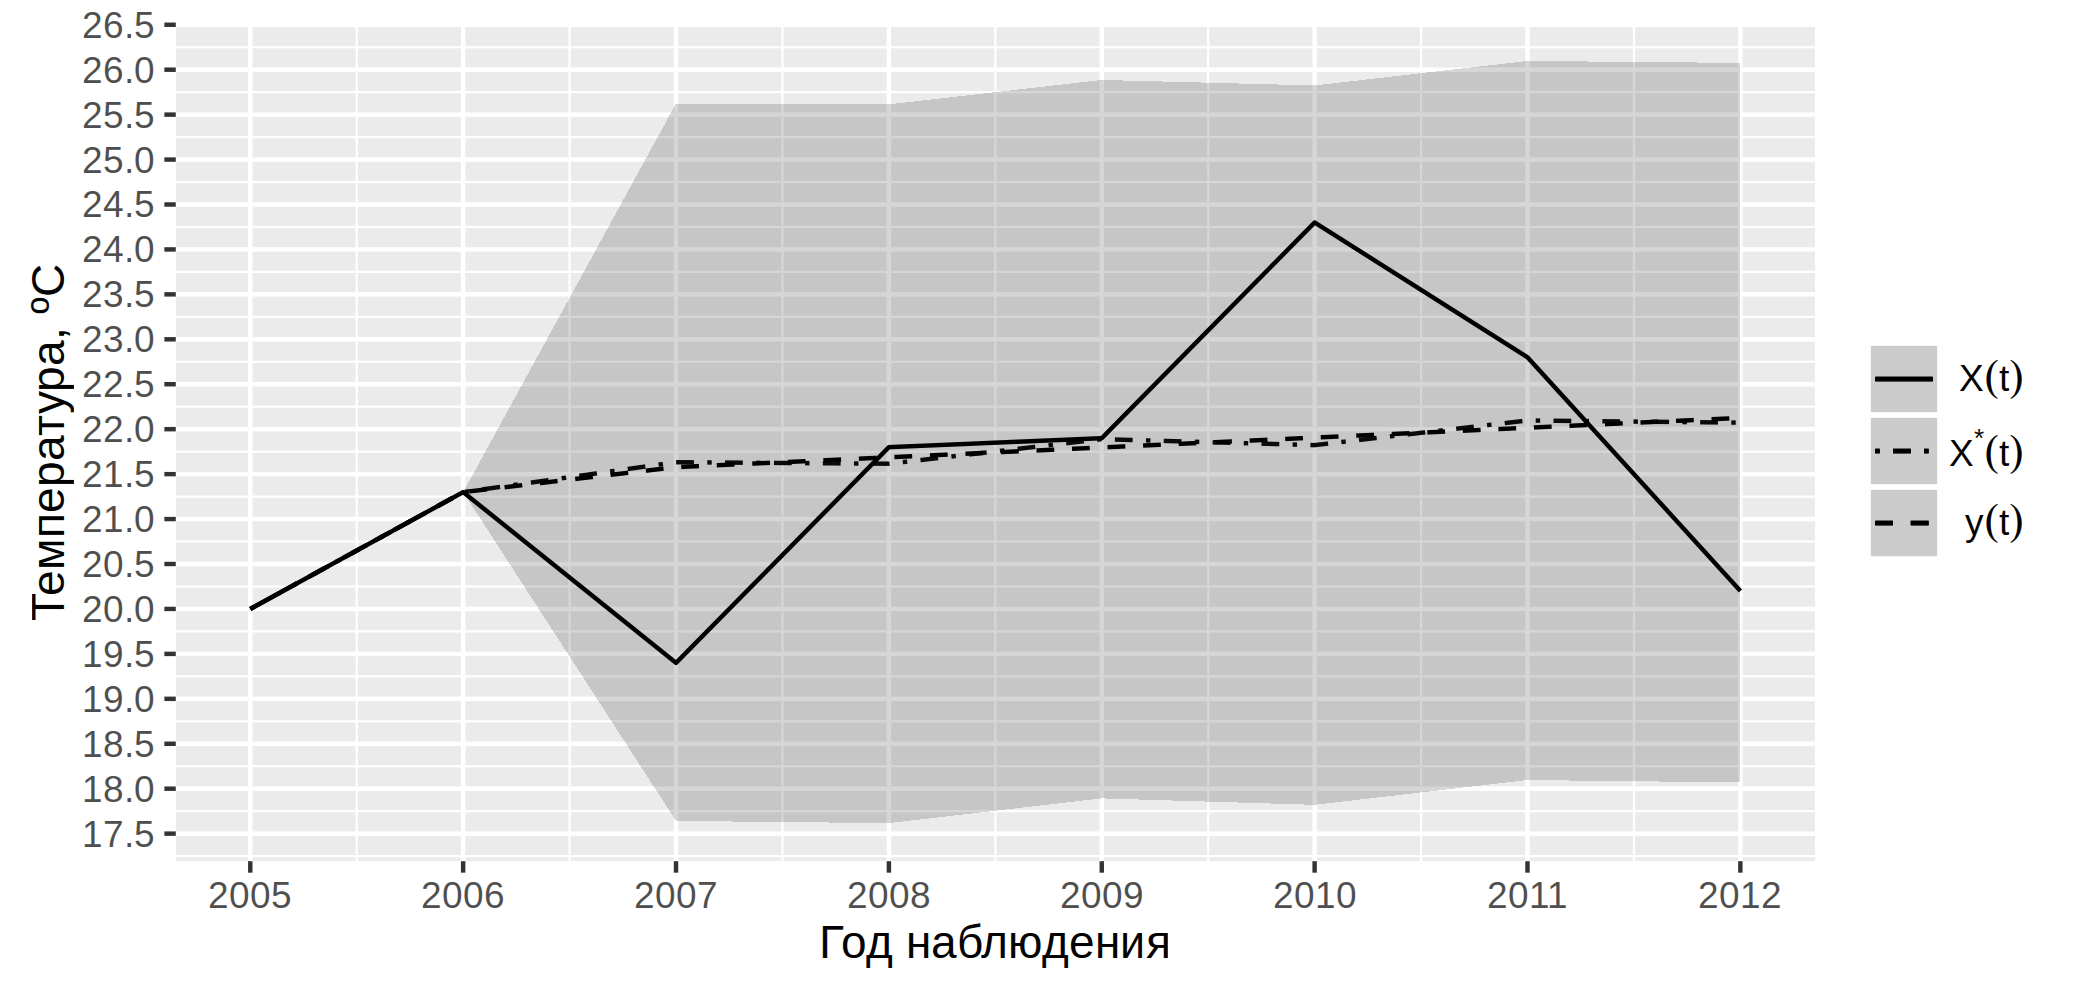
\includegraphics[width=0.8\linewidth]{../figures/variogram/auto-class-20-cross-prediction.png}}
\caption{Прогноз (модель $ \widehat{\gamma}_7(h) $)}
\label{img:auto-class-20-pred}
\end{figure}

\begin{figure}[H]
\center{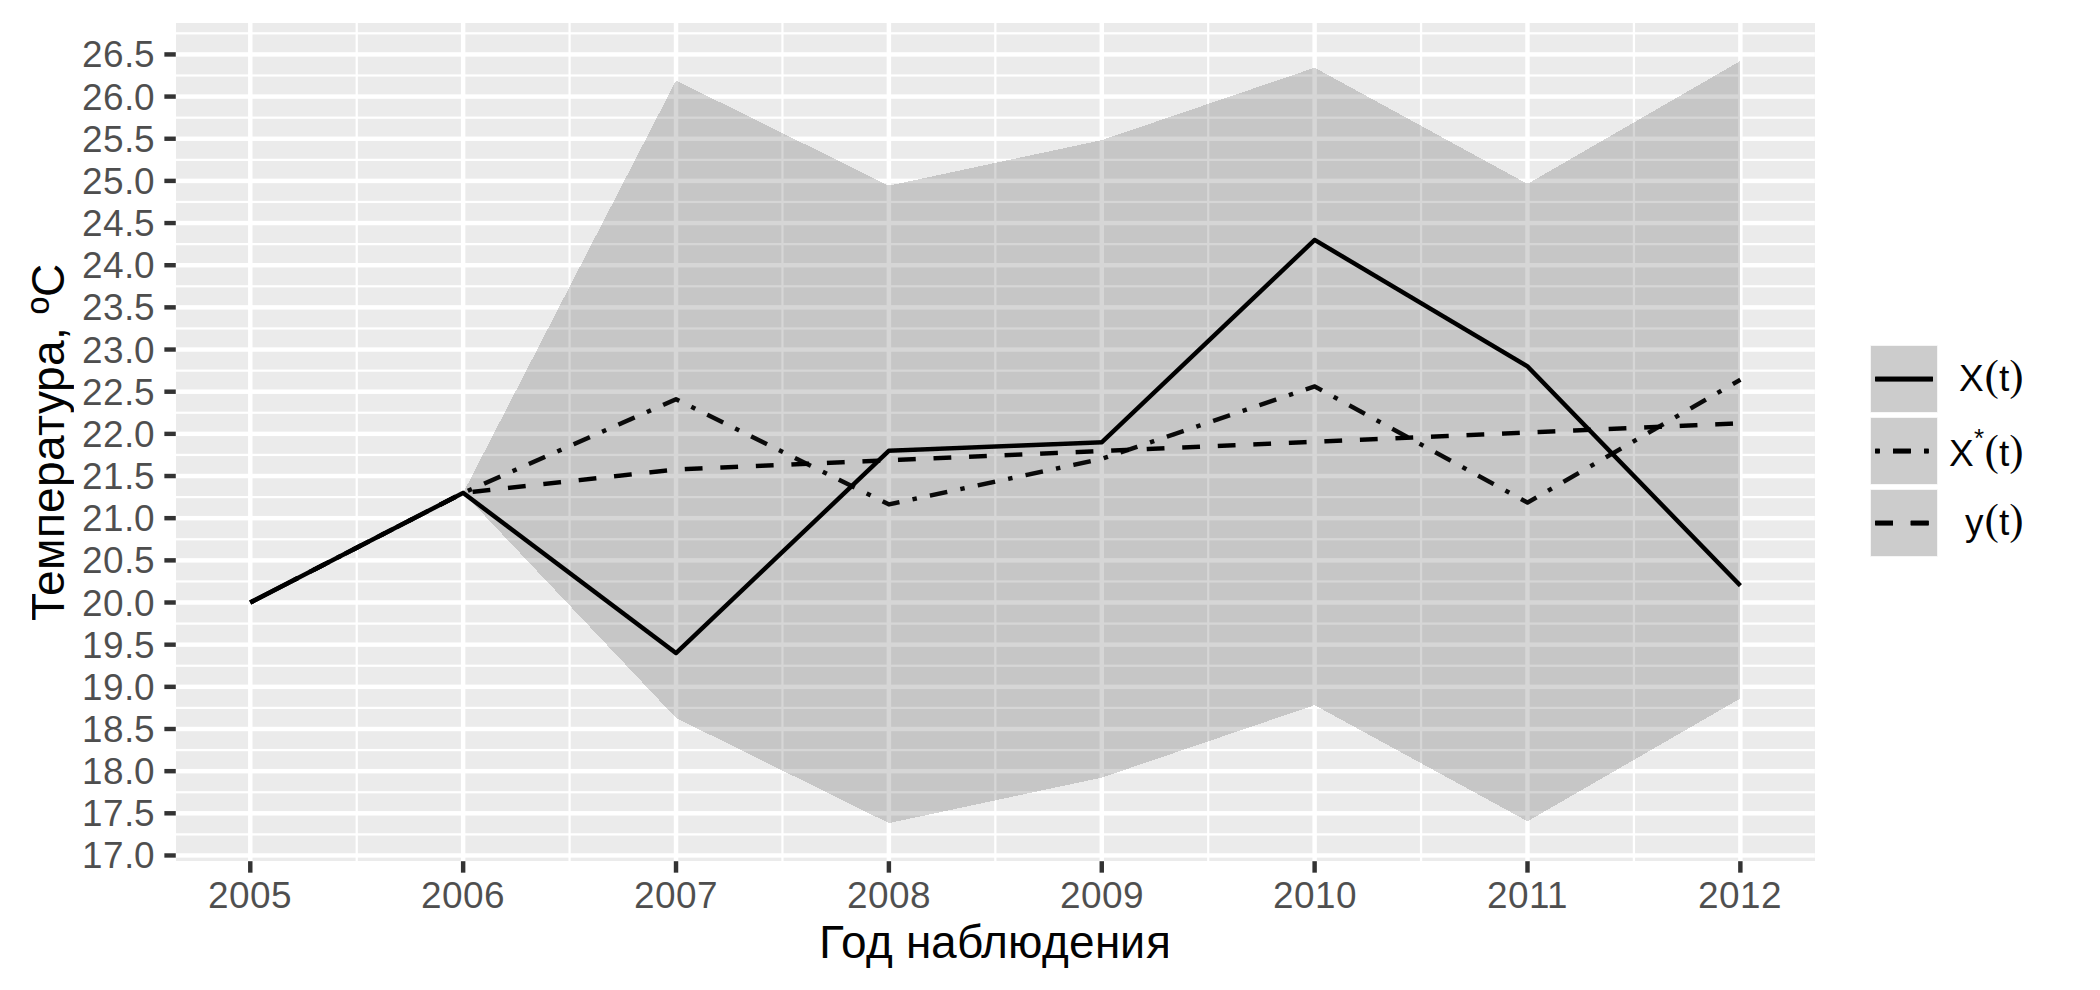
\includegraphics[width=0.8\linewidth]{../figures/variogram/auto-class-26-cross-prediction.png}}
\caption{Прогноз (модель $ \widehat{\gamma}_8(h) $)}
\label{img:auto-class-26-pred}
\end{figure}

\begin{figure}[H]
\center{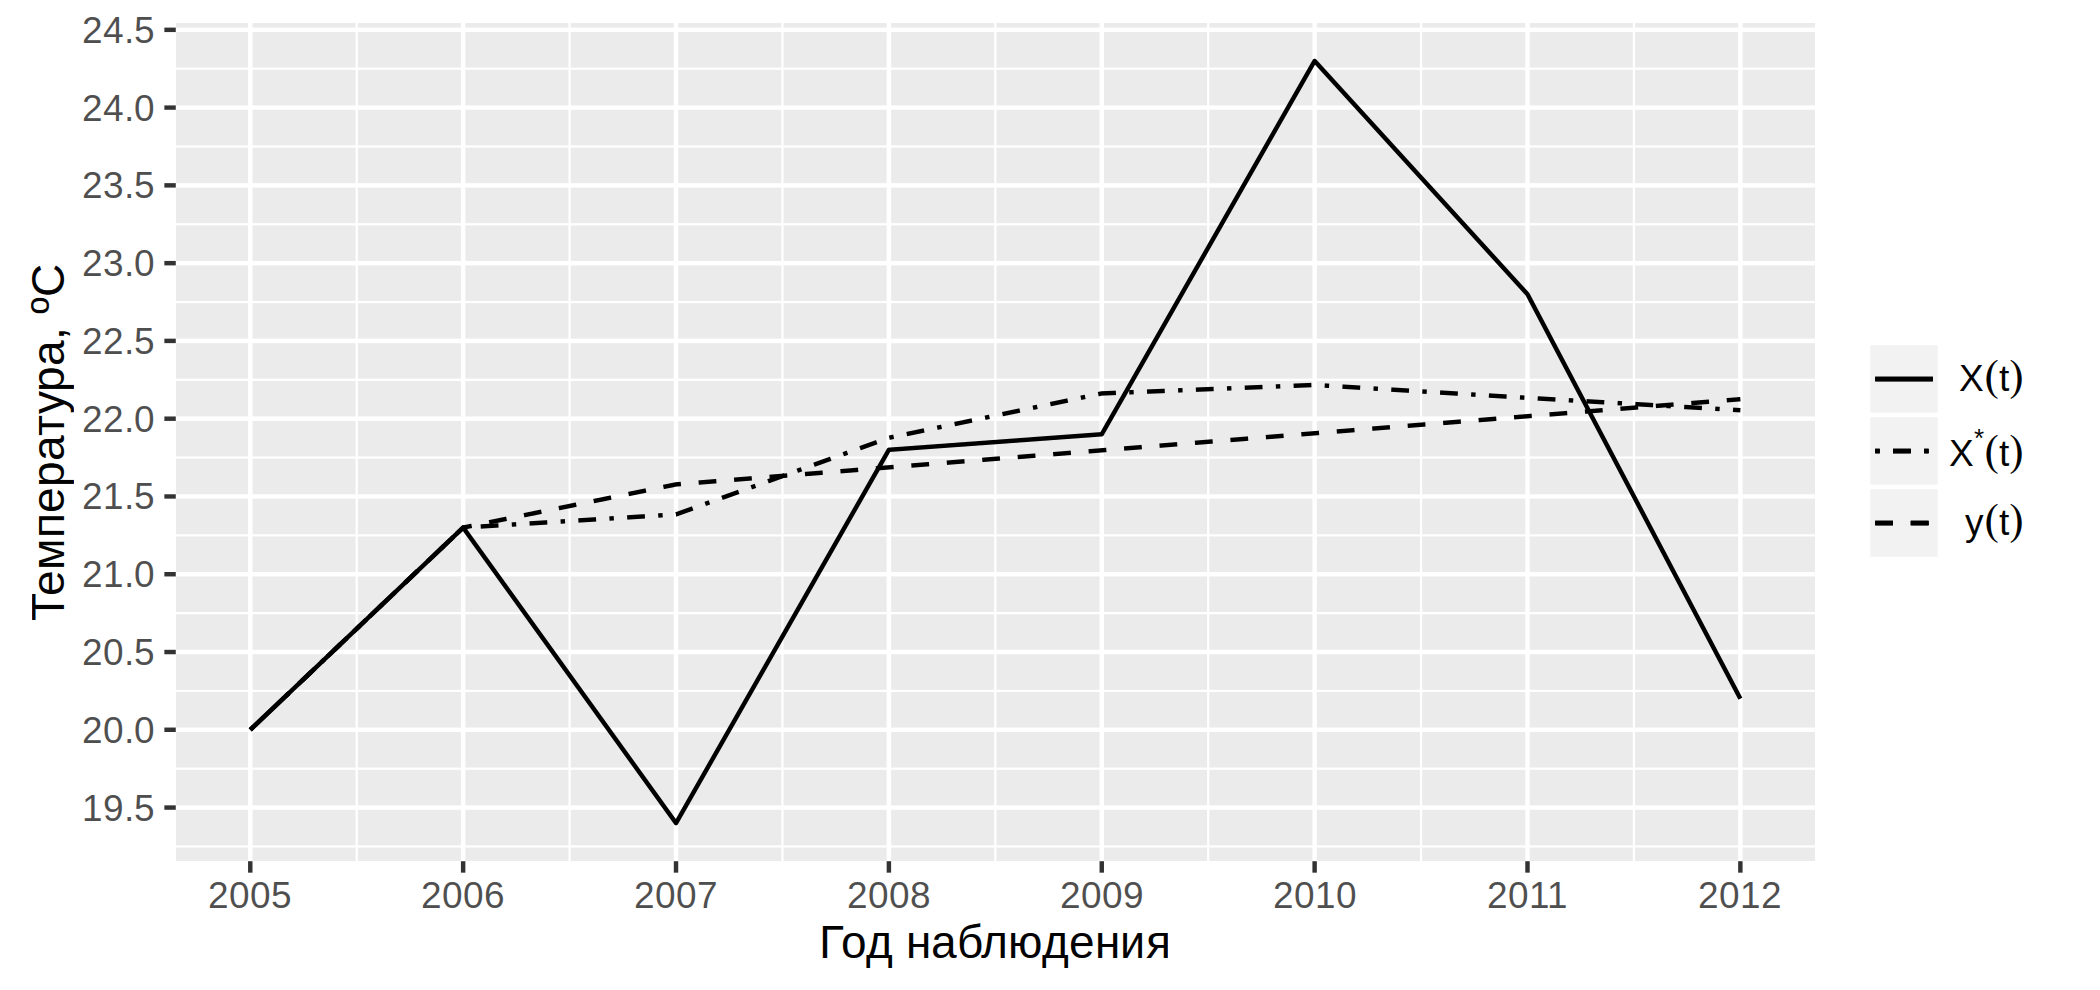
\includegraphics[width=0.8\linewidth]{../figures/variogram/auto-rob-5-cross-prediction.png}}
\caption{Прогноз (модель $ \widehat{\gamma}_9(h) $)}
\label{img:auto-rob-5-pred}
\end{figure}

\begin{figure}[H]
\center{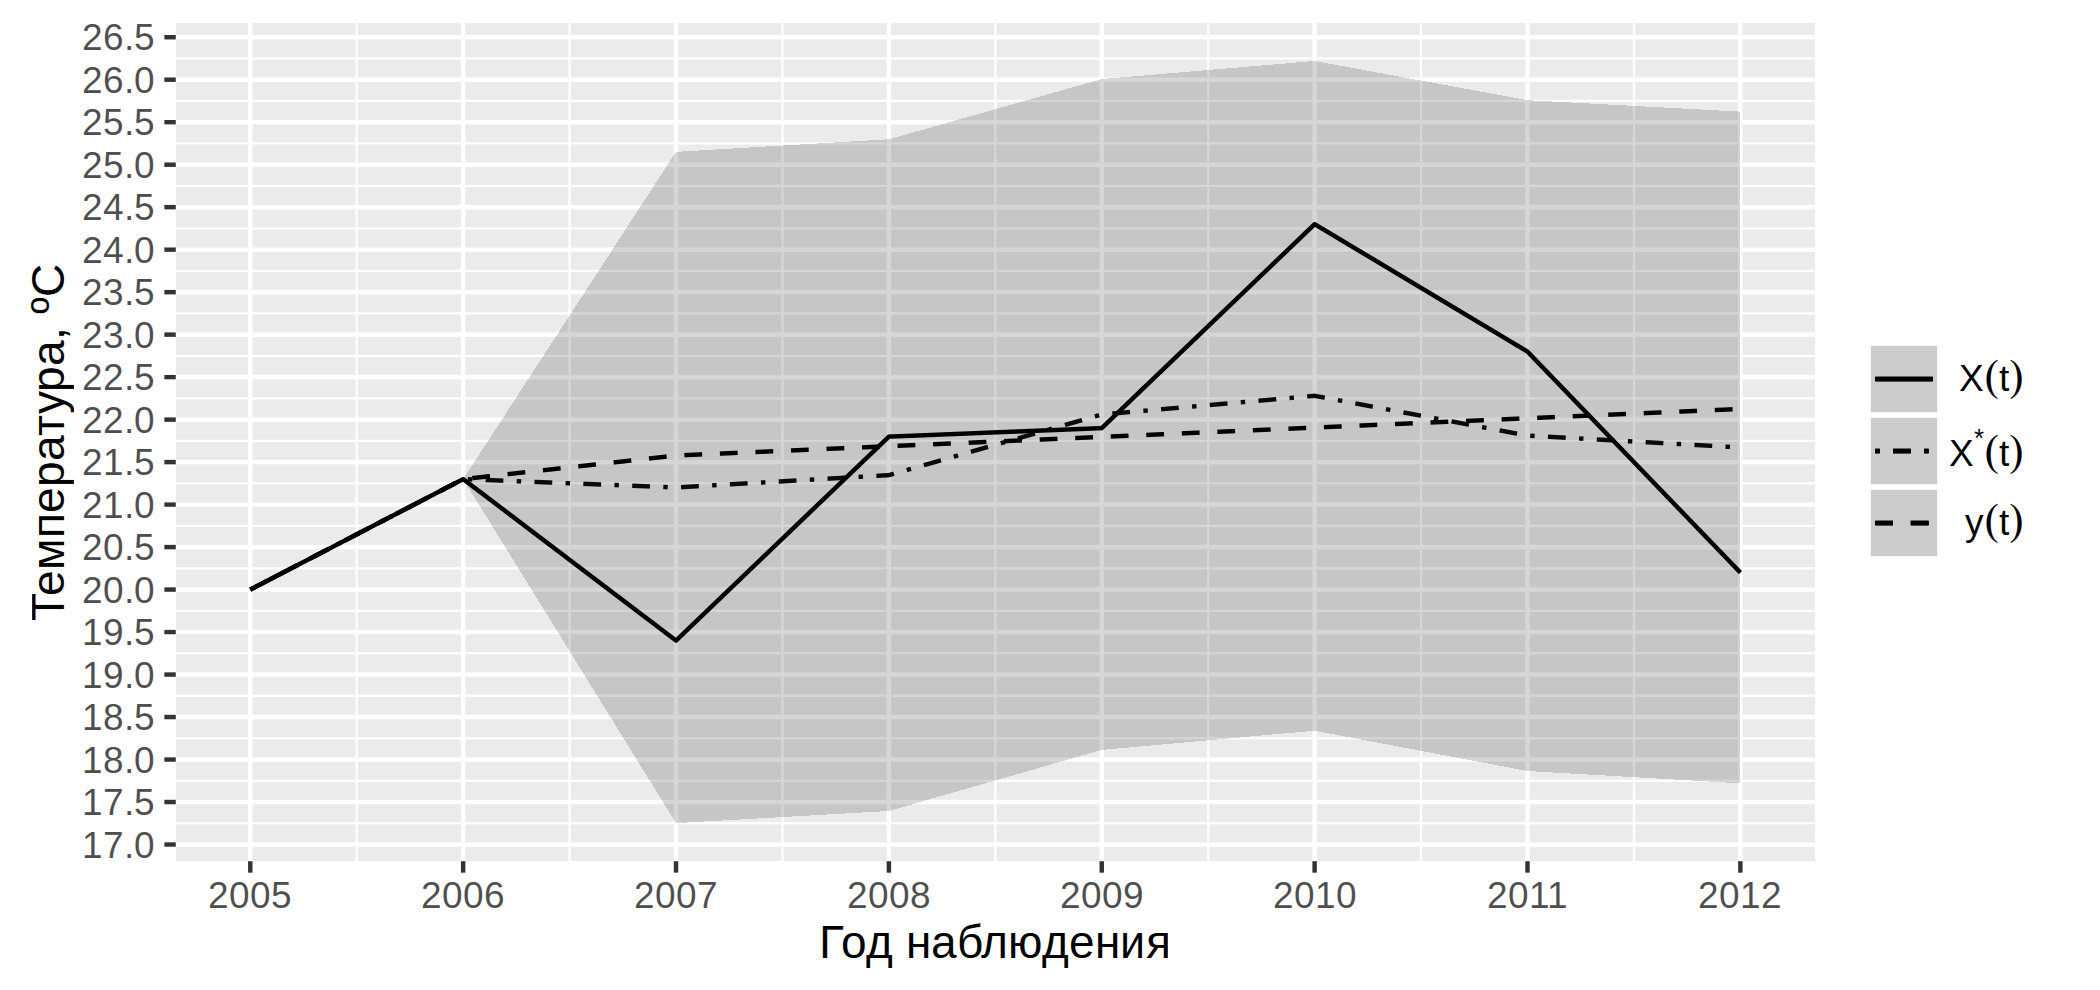
\includegraphics[width=0.8\linewidth]{../figures/variogram/auto-class-18-cross-prediction.png}}
\caption{Прогноз (модель $ \widehat{\gamma}_{10}(h) $)}
\label{img:auto-class-18-pred}
\end{figure}

\newpage
\section{ Результаты вычислений}
\label{c:app_results}

% latex table generated in R 3.1.2 by xtable 1.7-4 package
% Fri May 15 03:15:00 2015
\begin{table}[H]
\centering
\begin{tabular}{rrr}
  \hline
 & year & temperature \\ 
  \hline
1 & 1975.00 & 2.05 \\ 
  2 & 1976.00 & -2.25 \\ 
  3 & 1977.00 & -0.66 \\ 
  4 & 1978.00 & -1.71 \\ 
  5 & 1979.00 & -1.06 \\ 
  6 & 1980.00 & -1.89 \\ 
  7 & 1981.00 & 1.04 \\ 
  8 & 1982.00 & 0.14 \\ 
  9 & 1983.00 & 2.44 \\ 
  10 & 1984.00 & 0.33 \\ 
  11 & 1985.00 & 1.23 \\ 
  12 & 1986.00 & -2.77 \\ 
  13 & 1987.00 & -2.27 \\ 
  14 & 1988.00 & 4.33 \\ 
  15 & 1989.00 & 0.33 \\ 
  16 & 1990.00 & -1.17 \\ 
  17 & 1991.00 & 3.22 \\ 
  18 & 1992.00 & 2.02 \\ 
  19 & 1993.00 & -1.98 \\ 
  20 & 1994.00 & 1.32 \\ 
  21 & 1995.00 & -1.28 \\ 
  22 & 1996.00 & -1.18 \\ 
  23 & 1997.00 & 0.62 \\ 
  24 & 1998.00 & -2.09 \\ 
  25 & 1999.00 & 2.91 \\ 
  26 & 2000.00 & 0.31 \\ 
  27 & 2001.00 & 3.41 \\ 
  28 & 2002.00 & 2.21 \\ 
  29 & 2003.00 & -2.99 \\ 
  30 & 2004.00 & -1.99 \\ 
  31 & 2005.00 & -1.20 \\ 
  32 & 2006.00 & 0.00 \\ 
  33 & 2007.00 & -2.00 \\ 
  34 & 2008.00 & 0.30 \\ 
  35 & 2009.00 & 0.30 \\ 
   \hline
\end{tabular}
\caption{Временной ряд остатков.} 
\label{table:residuals}
\end{table}

% latex table generated in R 3.3.0 by xtable 1.8-2 package
% Tue Jun 21 13:42:40 2016
\begin{table}[H]
\centering
\caption{Прогнозные значения (модель $ \widehat{\gamma}_2(h) $)} 
\label{table:lin-fit-prediction}
\begin{tabular}{r|cccc}
  \hline
 & $X(t)$ & $X^{*}(t)$ & $y(t)$ & $ X(t) - X^{*}(t) $ \\ 
  \hline
2007 & 19.400 & 21.578 & 21.578 & -2.178 \\ 
  2008 & 21.800 & 21.687 & 21.687 & 0.113 \\ 
  2009 & 21.900 & 21.797 & 21.797 & 0.103 \\ 
  2010 & 24.300 & 21.906 & 21.906 & 2.394 \\ 
  2011 & 22.800 & 22.016 & 22.016 & 0.784 \\ 
  2012 & 20.200 & 22.126 & 22.126 & -1.926 \\ 
   \hline
\end{tabular}
\end{table}

% latex table generated in R 3.3.0 by xtable 1.8-2 package
% Tue Jun 21 13:42:42 2016
\begin{table}[ht]
\centering
\caption{Прогнозные значения (модель $ \widehat{\gamma}_4(h) $)} 
\label{table:lin-fit-adapt-prediction}
\begin{tabular}{r|cccc}
  \hline
 & $X(t)$ & $X^{*}(t)$ & $y(t)$ & $ X(t) - X^{*}(t) $ \\ 
  \hline
2007 & 19.400 & 19.427 & 21.578 & -0.027 \\ 
  2008 & 21.800 & 21.864 & 21.687 & -0.064 \\ 
  2009 & 21.900 & 21.974 & 21.797 & -0.074 \\ 
  2010 & 24.300 & 22.084 & 21.906 & 2.216 \\ 
  2011 & 22.800 & 22.193 & 22.016 & 0.607 \\ 
  2012 & 20.200 & 22.303 & 22.126 & -2.103 \\ 
   \hline
\end{tabular}
\end{table}

% latex table generated in R 3.1.3 by xtable 1.7-4 package
% Sat May 23 13:16:59 2015
\begin{table}[ht]
\centering
\begin{tabular}{rrrrrr}
  \hline
 & Год & Наблюдение & Прогноз & Тренд & Ошибка \\ 
  \hline
1 & 2007 & 19.400 & 22.133 & 21.578 & -2.733 \\ 
  2 & 2008 & 21.800 & 23.106 & 21.687 & -1.306 \\ 
  3 & 2009 & 21.900 & 23.441 & 21.797 & -1.541 \\ 
  4 & 2010 & 24.300 & 23.028 & 21.906 & 1.272 \\ 
  5 & 2011 & 22.800 & 22.122 & 22.016 & 0.678 \\ 
  6 & 2012 & 20.200 & 21.219 & 22.126 & -1.019 \\ 
   \hline
\end{tabular}
\caption{Прогноз (периодическая модель)} 
\label{table:per-fit-cv-prediction}
\end{table}

% latex table generated in R 3.1.3 by xtable 1.7-4 package
% Sat May 23 14:18:00 2015
\begin{table}[ht]
\centering
\begin{tabular}{rrrrrr}
  \hline
 & Год & Наблюдение & Прогноз & Тренд & Ошибка \\ 
  \hline
1 & 2007 & 19.400 & 21.385 & 21.578 & -1.985 \\ 
  2 & 2008 & 21.800 & 21.877 & 21.687 & -0.077 \\ 
  3 & 2009 & 21.900 & 22.163 & 21.797 & -0.263 \\ 
  4 & 2010 & 24.300 & 22.217 & 21.906 & 2.083 \\ 
  5 & 2011 & 22.800 & 22.134 & 22.016 & 0.666 \\ 
  6 & 2012 & 20.200 & 22.055 & 22.126 & -1.855 \\ 
   \hline
\end{tabular}
\caption{Прогноз (волновая модель)} 
\label{table:auto-rob-5-prediction}
\end{table}


\newpage
\section{ Код программы}
\label{c:listings}

\renewcommand{\thelstlisting}{Г.1}
\lstinputlisting[language=R, caption=Описательные статистики, label=lst:dstats]{../R/lib/dstats.R}
% \renewcommand{\thelstlisting}{Г.2}
% \lstinputlisting[language=R, caption=Основной код программы, label=lst:main]{../R/master.R}
\renewcommand{\thelstlisting}{Г.2}
% \lstinputlisting[language=R, caption=Вариограммный анализ, label=lst:variogram]{../R/predictor.R}
% \renewcommand{\thelstlisting}{Г.3}
% \lstinputlisting[language=R, caption=Автоматический подбор моделей, label=lst:afv]{../R/lib/afv.R}
